%\documentclass[handout]{beamer} %No effects
\documentclass{beamer} %Presentation effects
\usepackage{pgfpages}
%\pgfpagesuselayout{4 on 1}[a4paper,border shrink=5mm,landscape] %4 sided handout

\mode<presentation>
{
  \usetheme{cambridge}
  \setbeamertemplate{navigation symbols}{}
  \setbeamercovered{transparent}
}

\usepackage[english]{babel}
\usepackage[latin1]{inputenc}
\usepackage{multicol}

\title[An introduction to HPC on CSD3] % (optional, use only with long paper titles)
{An Introduction to High Performance Computing on the CSD3 Cluster}

\author[SJ Rankin & P Sumption] % (optional, use only with lots of authors)
{Paul sumption\\ \texttt{support@hpc.cam.ac.uk}}

\institute[UIS, University of Cambridge]
{Research Computing Services (http://www.hpc.cam.ac.uk/)\\
University Information Services (http://www.uis.cam.ac.uk/)}

\date[22/05/2018] % (optional)
{22nd May 2018 / CSD3 User Training}

\subject{Courses}

\begin{document}

\begin{frame}
  \titlepage
\end{frame}

\begin{frame}<presentation>{Welcome}
\begin{itemize}
\item{Please sign in on the {\color{red}attendance sheet}.}
\item Please fill in the {\color{red}online feedback} at the end of the course: There is a link to this on your desktop.
%      \url{http://feedback.training.cam.ac.uk/ucs/form.php}
\item{Keep your belongings with you.}
\item Course files can be downloaded from:  \url{www.csd3.cam.ac.uk}
\end{itemize}
\end{frame}

\begin{frame}<presentation>{Plan of the Course}
\begin{description}
\item[10:00] {Part 1: Course Introduction}
\item[10:15] {Part 2: HPC - Basic Concepts}
\item[11:00] {BREAK}
\item[11.20] {Part 3: HPC - Facilities}
\item[12:00] {Part 4: HPC - Connecting}
\item[13:00] {LUNCH}
\item[14:00] {Part 5: HPC - User Environment}
\item[15:00] {Part 6: HPC - Submission scripts}
\item[16:30] {FEEDBACK and CLOSE}
\medskip
\end{description}
\end{frame}

\part{Introduction}
\begin{frame}
\partpage
\end{frame}

%\begin{frame}{Basics: Outline}
%\small
%  \tableofcontents[subsectionstyle=hide]%[pausesections]
%\end{frame}

\section{Who are we?}
\begin{frame}{UIS: Research and Institutional Services Division}
Your trainers for today will be:\\
\begin{itemize}
  \item Paul Sumption --- Research Computing Technical Liaison
    \item Simon Flood --- Research Computing System Administrator
  \item Matthew Archer --- Research Software Engineering Team
  \item\alert{Please ask questions and let us know if you need assistance.}
\end{itemize}
\end{frame}

\section{Training Accounts}
\begin{frame}{Basics: Training accounts}
\begin{itemize}
\item{\alert{For our practical exercise's we will use HPC training accounts.}}
\pause
\item{You will find two pieces of paper on your desk.}
\pause
\item{1: A terms and conditions form for you to sign.}
\pause
\item{2: Your training account details.}
\pause
\item{Your training account will only be valid for today.}
\end{itemize}
\end{frame}

\section{Login node for today}
\begin{frame}{Basics: Login node}
\begin{itemize}
\item{\alert{For our practical exercise's we will use the login node: login-cpu.hpc.cam.ac.uk.}}
\pause
\item{Later in the course you will see that different nodes types may require you to use other login nodes.}
\end{itemize}
\end{frame}

\section{Security}
\begin{frame}{Basics: Security}
\begin{itemize}
\item{\alert{Boring but very, very important${}\ldots$}}
\pause
\item{Cambridge IT is under constant attack by would-be intruders.}
\pause
\item{Your data and research career is threatened by intruders.}
\pause
\item{\alert{Cambridge systems} are high profile and popular targets.}
\pause
\item{\alert{Don't let intruders in.}}
\end{itemize}
\end{frame}

\begin{frame}{Basics: Security}
\begin{enumerate}
\item{\alert{Keep your password (or private key passphrase) safe.}}
\pause
\item{\alert{Always choose strong passwords.}}
\pause
\item{\alert{Your UIS password is used for multiple systems so keep it secure!}}
\pause
\item{Keep the software on your laptops/tablets/PCs up to date this includes home computers especially if you are using the VPN to connect in.}
\pause
\item{Don't share accounts (this is against the rules anyway).}
\end{enumerate}
\end{frame}

\section{Basics: Pre-requisites}
\begin{frame}{Pre-requisites}
\begin{itemize}
\item{A pre-requisite of this course:}
\pause
\item{Basic Unix/Linux command line experience}
\item{\url{https://www.training.cam.ac.uk/ucs/Course/ucs-unixintro1} Unix: Introduction to the Command Line Interface (Self-paced)}
\pause
\item{Shell scripting experience is desirable}
\item{\url{https://www.training.cam.ac.uk/ucs/Course/ucs-scriptsci} Unix: Simple Shell Scripting for Scientists}
\end{itemize}
\end{frame}

\subsection{Navigating the command line }
\begin{frame}{Navigating your terminal}
Useful commands for navigating your terminal.
\begin{itemize}
\item{\alert{\footnotesize cd \textless dirname \textgreater } - change into a directory }
\item{\alert{\footnotesize ls \textless dirname \textgreater } - list the contents of a directory}
\item{\alert{\footnotesize cd or cd \path{~}} - change into your home folder}
\item{\alert{\footnotesize cd .. } - change back one folder}
\item{\alert{\footnotesize man ls } - will bring up the manual page for the ls command}
\item{\alert{\footnotesize pwd } - print working directory}
\end{itemize}
\end{frame}

\part{Basics}
\begin{frame}
\partpage
\end{frame}

\section{Why Buy a Big Computer?}

\begin{frame}{Basics: Why Buy a Big Computer?}

What types of big problem might require a ``Big Computer''?

\begin{description}
\pause
\item[\textit{Compute Intensive:}]{A single problem requiring a large amount of computation.}
\pause
\item[\textit{Memory Intensive:}]{A single problem requiring a large amount of memory.}
\pause
\item[\textit{Data Intensive:}]{A single problem operating on a large amount of data.}
\pause
\item[\textit{High Throughput:}]{Many unrelated problems to be executed in bulk.}
\end{description}
\end{frame}

\begin{frame}{Basics: Compute Intensive Problems}
\begin{itemize}
\item{Distribute the \alert{work} for a \alert{single problem} across multiple CPUs to reduce the execution time as far as possible.}
\pause
\item{Program workload must be \emph{parallelised}:}
\begin{description}
\item{Parallel programs split into copies (processes or threads).}
\item{Each process/thread performs a part of the work on its own CPU, concurrently with the others.}
\item{A well-parallelised program will fully exercise as many CPUs as there are processes/threads.}
\end{description}
\pause
\item{The CPUs typically need to exchange information rapidly, requiring specialized communication hardware.}
\pause
\item{Many use cases from Physics, Chemistry, Engineering, Astronomy, Biology...}
\item{The traditional domain of \alert{HPC} and the \alert{Supercomputer}.}
\end{itemize}
\end{frame}

\begin{frame}{Basics: Scaling \& Amdahl's Law}
\begin{itemize}
\item{\alert{Using more CPUs is not necessarily faster.}}
  \pause
\item{Typically parallel codes have a \alert{scaling limit}.}
\item{Partly due to the system overhead of managing more copies, but also to more basic constraints;}
\pause
\item{Amdahl's Law (idealized):}
\[
S(N)=\frac{1}{\left(1-p+\frac{p}{N}\right)}
\]
where \begin{align*}S(N)&\text{ is the fraction by which the program has sped up}\\&\text{ relative to $N=1$}\\
p&\text{ is the fraction of the program which can be parallelized}\\
N&\text{ is the number of CPUs.}
\end{align*}
\end{itemize}
\end{frame}

\begin{frame}{Basics: Amdahl's Law}
\centerline{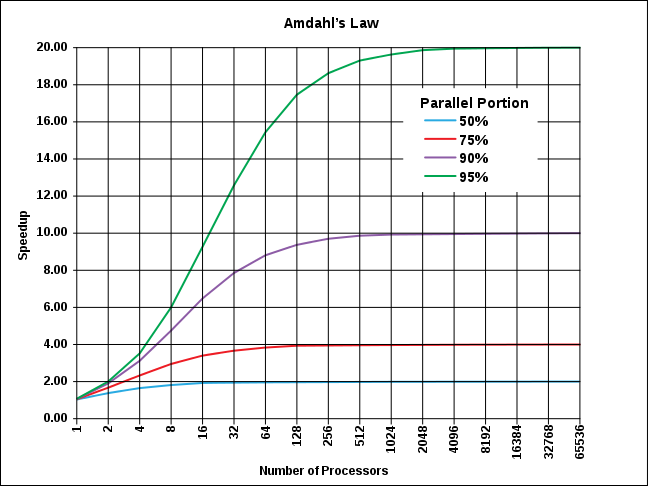
\includegraphics[width=0.75\textwidth]{imgs/AmdahlsLaw.png}}%
\rightline{\tiny http://en.wikipedia.org/wiki/File:AmdahlsLaw.svg}
\smallskip
\end{frame}

\begin{frame}{The Bottom Line}
\begin{itemize}
\item{Parallelisation requires effort:}
\begin{itemize}
\item{There are libraries to help (e.g. \alert{OpenMP}, \alert{MPI}).}
\item{First optimise performance on one CPU, then make $p$ as large as possible.}
\end{itemize}
\pause
\item{The scaling limit: eventually using more CPUs becomes \alert{detrimental} instead of helpful.}
\end{itemize}
\end{frame}

\begin{frame}{Basics: Data Intensive Problems}
\begin{itemize}
\item{Distribute the \alert{data} for a \alert{single problem} across multiple CPUs to reduce the overall execution time.}
\pause
\item{The \emph{same} work may be done on each data segment.}
\pause
\item{Rapid movement of data to and from disk is more important than inter-CPU communication.}
\pause
\item{\alert{Big Data} problems of great current interest -}
\item{Hadoop/MapReduce}
\item{Life Sciences (genomics) and elsewhere.}
\end{itemize}
\end{frame}

\begin{frame}{Basics: High Throughput}
\begin{itemize}
\item{Distribute \alert{independent}, \alert{multiple problems} across multiple CPUs to reduce the overall execution time.}
\pause
\item{Workload is trivially (or \emph{embarrassingly}) parallel:}
\begin{itemize}
\item[$\ast$]{Workload breaks up naturally into \emph{independent} pieces.}
\item[$\ast$]{Each piece is performed by a separate process/thread on a separate CPU (concurrently).}
\item[$\ast$]{\alert{Little or no inter-CPU communication}.}
\end{itemize}
\pause
\item{Emphasis is on throughput over a period, rather than on performance on a single problem.}
\pause
\item{Compute intensive capable $\Rightarrow$ high throughput capable}
\pause
\item{\color{red}Compute intensive capable $\not\Leftarrow$ high throughput capable} 
\end{itemize}
\end{frame}

\begin{frame}{Basics: Memory Intensive Problems}
\begin{itemize}
\item{Require aggregation of large memory into a \alert{single system image} (i.e.\ a single computer running Linux).}
%\pause
%\begin{description}
%\item{\alert{NB Memory (fast, volatile) not disk (slow, non-volatile).}}
%\end{description}
\pause
\item{Technically more challenging to build machines (very fast, low latency interconnection between \alert{all} CPUs and \alert{all} memory).}
\pause
\item{Coding/porting easier (memory appears seamless).}
\pause
\item{Optimisation harder (memory is actually highly nonuniform).}
\pause
\item{Historically, the arena of large \alert{SGI} systems.}
\pause
\item{Nowadays, similar complexity inside single commodity servers.}
\end{itemize}
\end{frame}


\section{Inside a Modern Computer}
\begin{frame}{Basics: Inside a Modern Computer}{CPUs in a box}
\only<1-7>{%
\begin{itemize}
\item<1-7>{Today's commodity servers already aggregate both CPUs and memory to make a single system image in a single box.}
\item<2-7>{Even small computers now have multiple CPU cores per socket\hfill\\
\visible<3-7>{\alert{$\implies{}$each socket is a Symmetric Multi-Processor (SMP).}}}
\item<4-7>{Larger computers have multiple sockets (each with local memory):\hfill\\
{}\qquad all CPU cores (unequally) share the node memory\hfill\\
{}\qquad \visible<5-7>{$\implies{}$the node is a \alert{shared memory} multiprocessor}\\
{}\qquad \visible<6-7>{with Non-Uniform Memory Architecture (\alert{NUMA})}\\
{}\qquad \visible<7>{but users still see a single computer (\alert{single system image}).}}
\end{itemize}
}%
\end{frame}

\begin{frame}{Basics: Inside a Modern Computer}{CPUs in a box}
\centerline{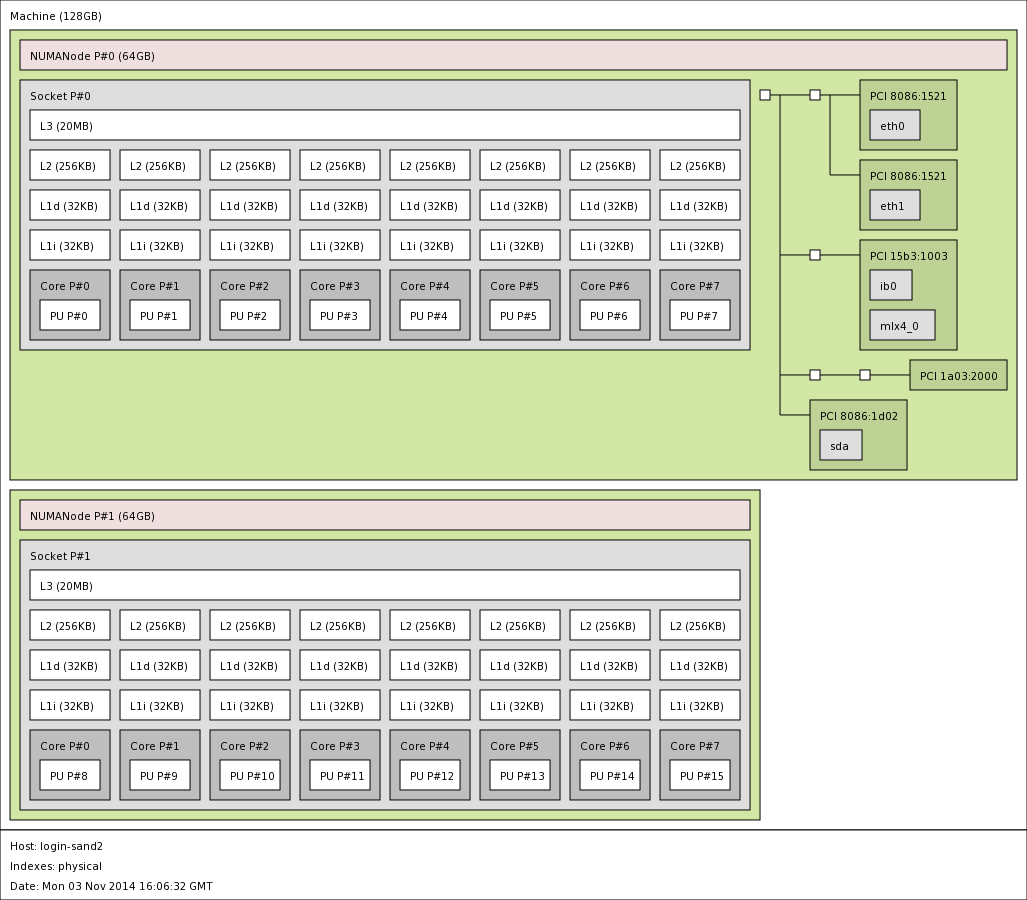
\includegraphics[width=0.8\textwidth]{imgs/lstopo.png}}
\end{frame}

\section{How to Build a Supercomputer}
\begin{frame}{Basics: How to Build a Supercomputer}
\only<1,2>{\begin{itemize}
\item{A supercomputer aggregates contemporary CPUs and memory to obtain increased computing power.}
\pause
\item{Usually today these are \alert{clusters}.}
\end{itemize}}
\only<3->{\begin{enumerate}
\item{Take some (multicore) CPUs plus some memory.}
\begin{itemize}
\item<4->{Could be an off-the-shelf server, or something more special.}
\item<5->{A NUMA, shared memory, multiprocessor building block: a \alert{node}.}
\end{itemize}
\end{enumerate}
}
\end{frame}


\begin{frame}{Basics: How to Build a Supercomputer}
\begin{tabular}{ll}
\parbox[c]{0.5\textwidth}{\begin{enumerate}
\setcounter{enumi}{1}
\item{Connect the nodes with one or more \alert{networks}.}
\pause
\null\par
Faster network for \alert{inter-CPU communication across nodes}.\par
Slower network for \alert{management} and \alert{provisioning}.\par
\alert{Storage} may use either.
\end{enumerate}}
&\vbox to 0pt{\vss\vskip 0.25cm\leftline{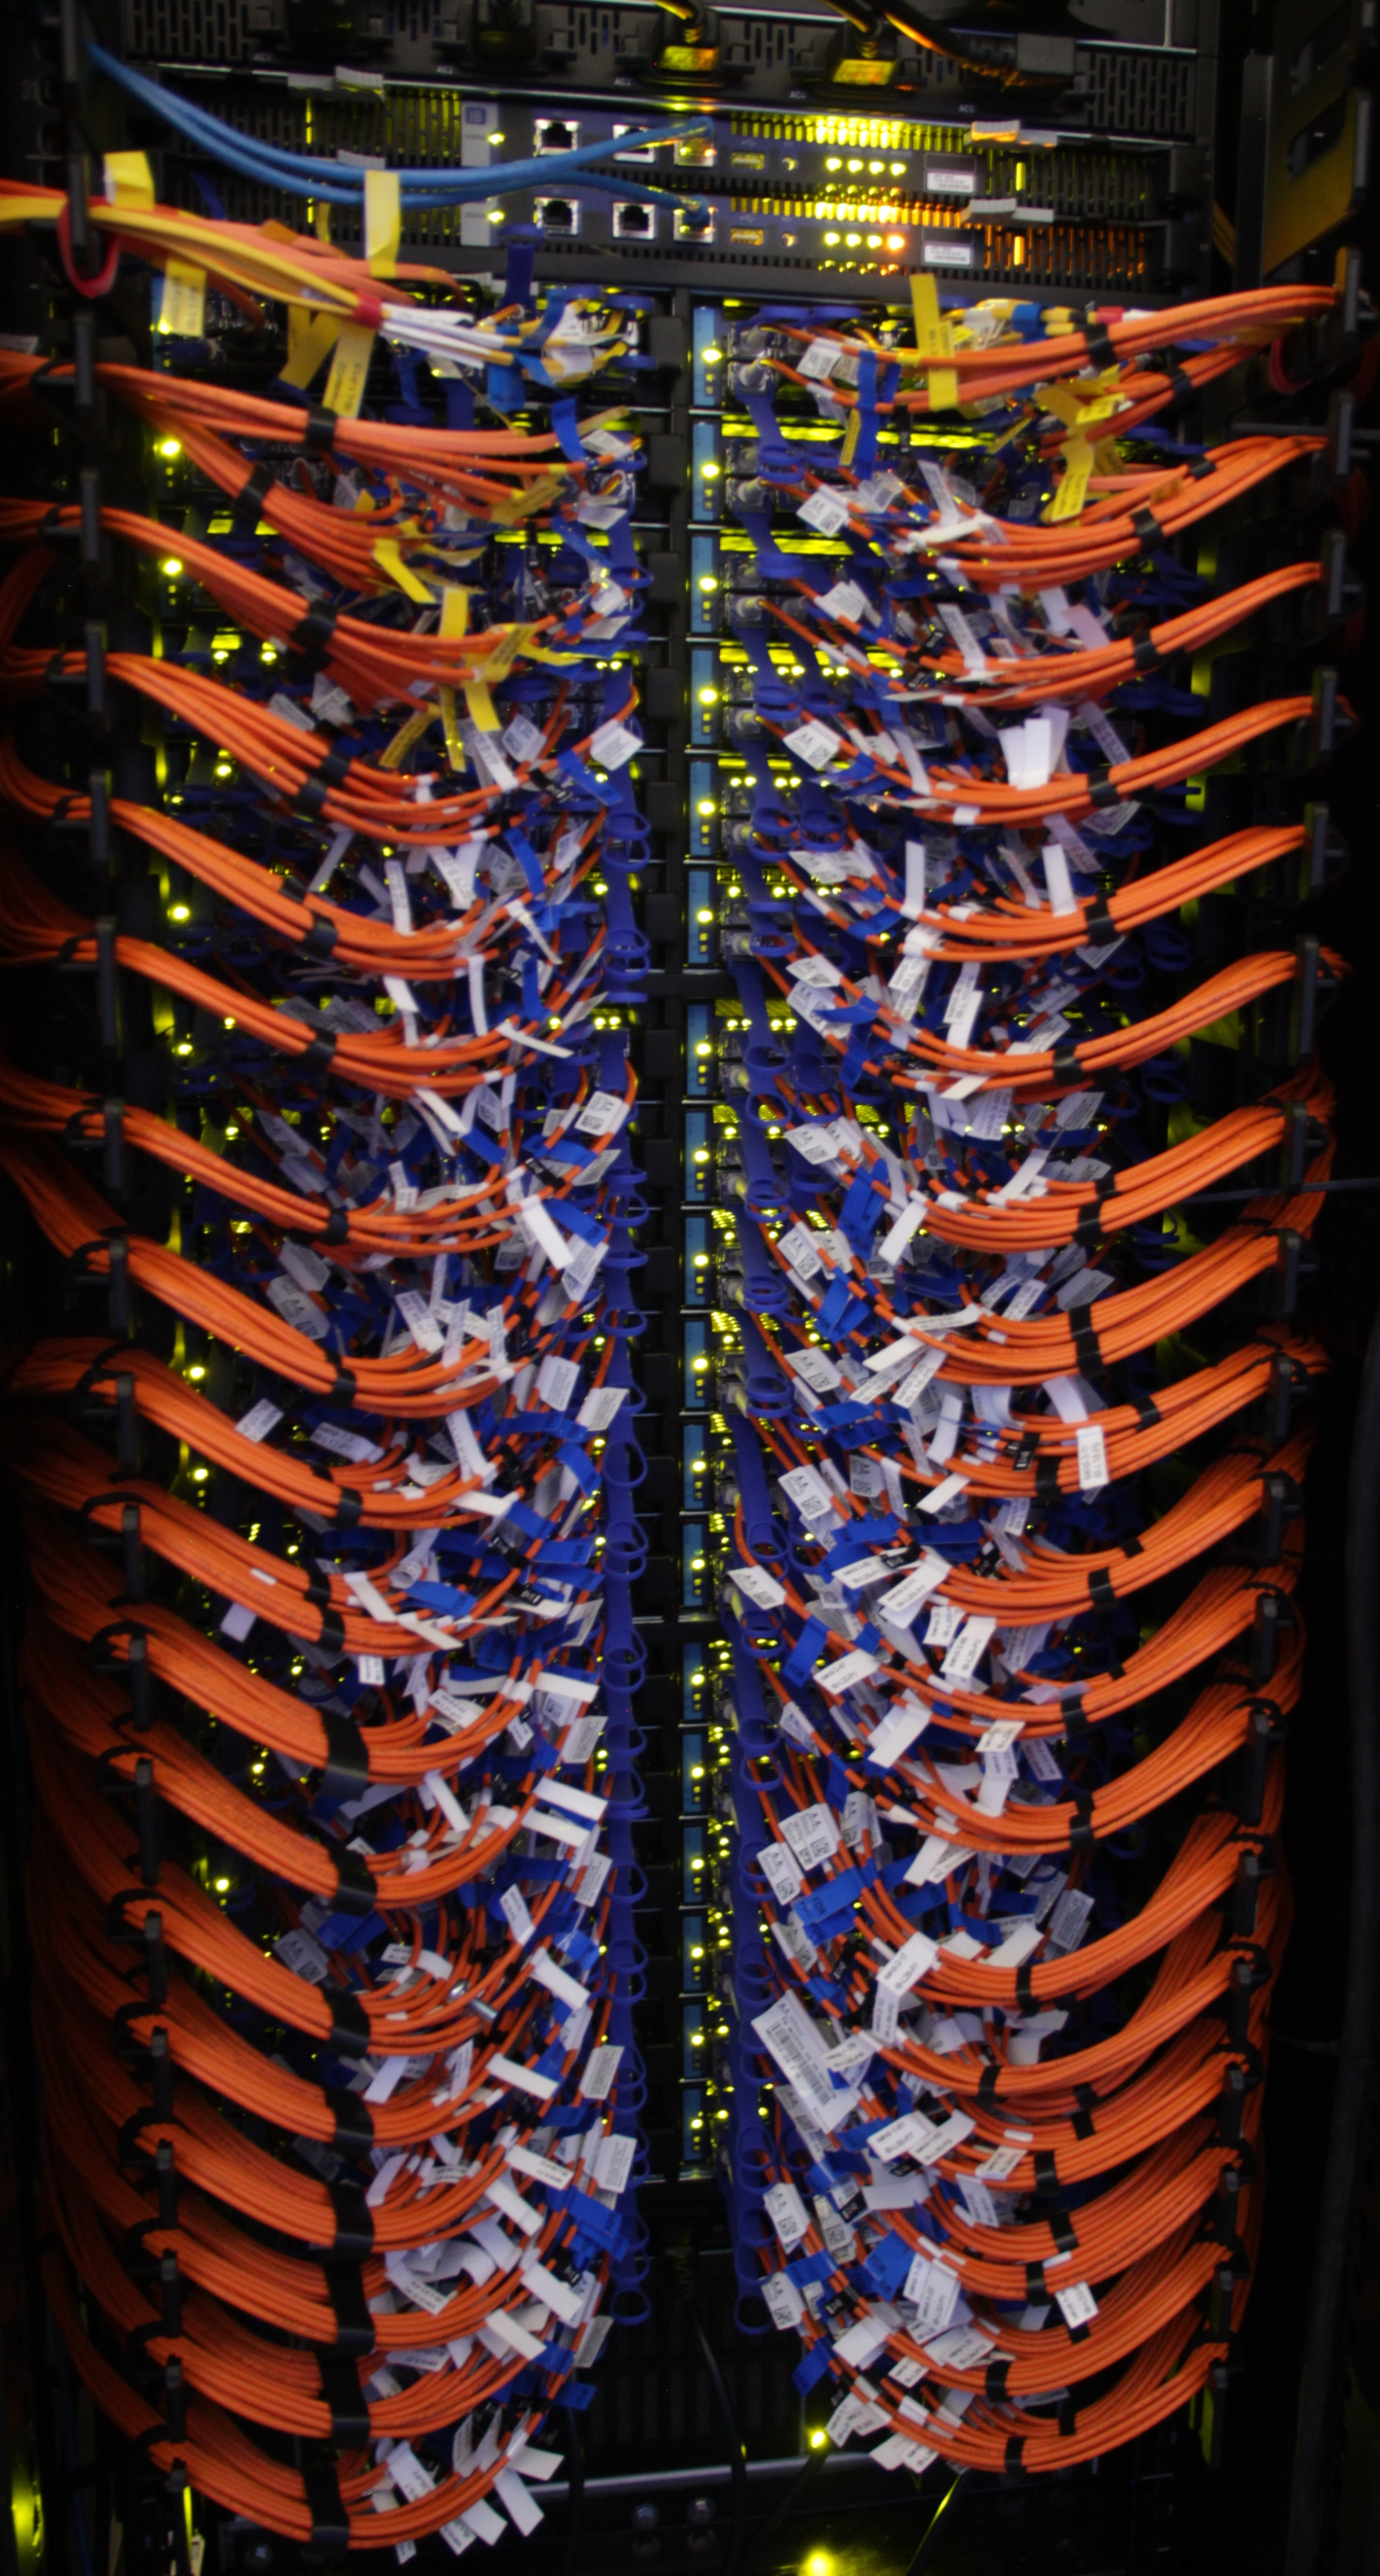
\includegraphics[height=0.85\textheight]{imgs/coreib.jpg}}\vss}\\
\end{tabular}
\end{frame}

\begin{frame}{Basics: How to Build a Supercomputer}
\begin{enumerate}
\setcounter{enumi}{2}
\item{Logically bind the nodes}
\begin{itemize}
\item{Clusters consist of distinct nodes (i.e. separate Linux computers)\hfill\\
on common private network(s) and controlled centrally.}
\begin{itemize}
\item[$\ast$]{Private networks allow CPUs in different nodes to communicate.}
\pause
\item[$\ast$]{Clusters are \alert{distributed memory} machines:\hfill\\
\alert{Each process/thread sees only its local node's CPUs and memory (without help).}}
\pause
\item[$\ast$]{\color{red}Each process/thread must fit within a single node's memory.}
\end{itemize}

%\pause
%\item{More expensive machines logically bind nodes into a single system\hfill\\
%{}\qquad i.e. CPUs \alert{and} memory.}
%\begin{itemize}
%\item[$\ast$]{E.g.\ SGI UV.}
%\item[$\ast$]{Private networks allow CPUs to see CPUs and memory in other nodes.}
%\pause
%\item[$\ast$]{These are \alert{shared memory} machines.}
%\item[$\ast$]{Logically a single system - 1 big node - but very non-uniform.}
%\item[$\ast$]{A single process can span the entire system.}
%\end{itemize}
\end{itemize}
\end{enumerate}

\end{frame}

\section{Programming a Multiprocessor Machine}
\begin{frame}{Basics: Programming a Multiprocessor Machine}
\only<1-3>{\begin{itemize}
\item{Non-parallel (serial) code}
\begin{itemize}
\item[$\ast$]{\alert{For a single node as for a workstation.}}
\pause
\item[$\ast$]{Typically \alert{run as many copies per node as CPUs}, assuming node memory is sufficent.}
\pause
\item[$\ast$]{\alert{Replicate across multiple nodes.}}
\end{itemize}
\end{itemize}}
\only<4->{\begin{itemize}
\item{Parallel code}
\begin{itemize}
\item<5->[$\ast$]{\alert{Shared memory methods within a node.}\hfill\\
E.g. pthreads, OpenMP.}
\item<6->[$\ast$]{\alert{Distributed memory methods spanning multiple nodes.}\hfill\\
Message Passing Interface (MPI).}
\end{itemize}
\end{itemize}}

\end{frame}

\section{Summary}

\begin{frame}{Basics: Summary}

  \begin{itemize}
  \item<1->{\alert{Why have a supercomputer?}}
  \begin{itemize}\item<2->{Big single problems, many problems, Big Data.}\end{itemize}
  \item<3->{Most current supercomputers are \alert{clusters} of separate \alert{nodes}.}
  \item<4->{Each node has \alert{multiple CPUs} and \alert{non-uniform shared memory}.}
  \item<5->{\alert{Parallel} code uses shared memory (\alert{pthreads/OpenMP}) within a node, distributed memory (\alert{MPI}) spanning multiple nodes.}
  \item<6->{\alert{Non-parallel} code uses the memory of one node, but may be copied across many.}
  \end{itemize}
  \end{frame}


\part{HPC Facilities}
\begin{frame}
\partpage
\end{frame}

\section{CSD3}
\begin{frame}{CSD3 - University of Cambridge}
\begin{itemize}
\item{Cambridge Service for Data Driven Discovery}
\pause
\medskip
\item{\alert{Peta4 --- Intel CPU cluster}}
\pause
\item{\alert{Wilkes2 --- NVIDIA GPU cluster}}
\pause
\medskip
\item{Hadoop-based data analytic platform}
\item{Burst buffer}
\item{Industry users through CORE.}
\end{itemize}
\end{frame}

\section{Peta4-Skylake}
\begin{frame}{Peta4-Skylake}
\begin{itemize}
\item{Each compute node:}
\begin{itemize}
\item[$\ast$]{\only<1>{2x16 cores, Intel Skylake 2.6 GHz}\only<2->{{\color{red}32 CPUs}}}
\item[$\ast$]{\only<1>{$192\,\text{GB}$ or $384\,\text{GB}$ RAM}\only<2->{{\color{red}$6\,\text{GB}$ or $12\,\text{GB}$ per CPU}}}
\item[$\ast$]{\only<1>{$100\,\text{Gb/sec}$ Omni-Path}\only<2->{\color{red}$10\,\text{GB/sec}$ (for MPI and storage)}}
\end{itemize}
\item{768 compute nodes}
\item{8 login nodes (\alert{login-cpu.hpc.cam.ac.uk})}
\end{itemize}
\end{frame}

%\section{Coprocessors --- GPUs etc}
%\begin{frame}{Coprocessors --- GPUs etc}
%  \begin{itemize}
%  \item{CPUs are \alert{general purpose}}
%    \pause
%  \item{Some types of parallel workload fit \alert{vector} processing well:}
%    \begin{itemize}
%    \item{Single Instruction, Multiple Data (SIMD)}
%    \item{\emph{Think pixels on a screen}}\pause
%    \item{GPUs specialise in this type of work}\pause
%      \item{Also competitor many-core architectures such as the Intel Phi}
%    \end{itemize}
%\end{itemize}
%\end{frame}

\section{Wilkes2-GPU}
\begin{frame}{Wilkes2-GPU}
\begin{itemize}
\item{Each compute node:}
\begin{itemize}
\item[$\ast$]{\only<1>{$4\times\text{NVIDIA P100 GPU}$}\only<2->{\color<2->{red}4 GPUs}}
\item[$\ast$]{\only<1>{1x12 cores, Intel Broadwell 2.2 GHz}\only<2->{{\color{red}12 CPUs}}}
\item[$\ast$]{\only<1>{$96\,\text{GB}$ RAM}\only<2->{{\color{red}$96\,\text{GB}$ RAM}}}
\item[$\ast$]{\only<1>{$100\,\text{Gb/sec}$ (4X EDR) Infiniband.}\only<2->{\color{red}$10\,\text{GB/sec}$ (for MPI and storage)}}
\end{itemize}
\item{90 compute nodes.}
\item{8 login nodes (\alert{login-gpu.hpc.cam.ac.uk}).}
\end{itemize}
\end{frame}

\section{Peta4-KNL}
\begin{frame}{Peta4-KNL (Intel Phi)}
\begin{itemize}
\item{Each compute node:}
\begin{itemize}
\item[$\ast$]{\only<1>{64 cores, Intel Phi 7210}\only<2->{{\color{red}256 CPUs}}}
\item[$\ast$]{\only<1>{$96\,\text{GB}$ RAM}\only<2->{{\color{red}$96\,\text{GB}$ RAM}}}
\item[$\ast$]{\only<1>{$100\,\text{Gb/sec}$ Omni-Path}\only<2->{\color{red}$10\,\text{GB/sec}$ (for MPI and storage)}}
\end{itemize}
\item{342 compute nodes}
\item{Shared login nodes with Peta4-Skylake}
\end{itemize}
\end{frame}


%\begin{frame}{HPCS Production Cluster Schematic}
%\centerline{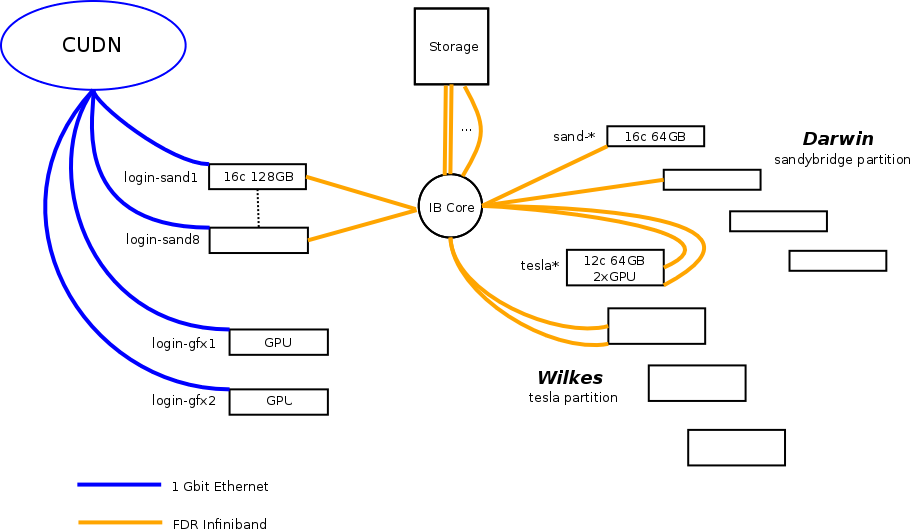
\includegraphics[width=0.95\textwidth]{imgs/cluster.png}}%
%\end{frame}

\section{Storage}
\begin{frame}{HPCS: Storage}
\begin{itemize}
\item{Multi-petabytes split across multiple filesystems with tape.}
\item{Lustre cluster filesystem:}
\begin{itemize}
\item[$\ast$]{Multiple RAID6 back-end disk volumes.}
\item[$\ast$]{Multiple object storage servers.}
\item[$\ast$]{Single metadata server.}
\item[$\ast$]{Tape-backed HSM on newest filesystems.}
\pause
\item[$\ast$]{\alert{$4\,\text{GB/sec}$ overall read or write.}}
\pause
\item[$\ast$]{\alert{Prefers big read/writes over small.}}
\end{itemize}
\pause
\item{\alert{For active HPC work only.}}
\end{itemize}
\end{frame}

\section{Obtaining an Account and Support}
\begin{frame}{Obtaining an Account and Support}
\begin{itemize}
\item{To apply for an account, complete our online form:}
\item \small {\url{https://www.csd3.cam.ac.uk/services/applying-for-resources}}
\pause
\item{For support enquiries please email our Service Desk:}
\item{\alert{support@hpc.cam.ac.uk}}
\end{itemize}
\end{frame}
\part{Using HPC}
\begin{frame}
\partpage
\end{frame}

\section{Connecting}
\begin{frame}{Basics: Connecting}
\begin{itemize}
\item When connecting to the cluster will we use the SSH secure protocol only.
\item We will use the Linux workstations during this course
\item Please check your workstation is booted into Ubuntu Linux, ask if you need help with this.
\item You are welcome to use your own laptop, however you may need to install some software in order to connect.
\item Later in this section of the slides we will cover the software you may need to install on your own computer.
\end{itemize}
\end{frame}

\subsection{Connecting - SSH}
\begin{frame}{Basics: Connecting}
\begin{itemize}
\item SSH secure protocol only.\hfill\\
\visible<2->{\alert{Supports login, file transfer, remote desktop\ldots}}
\item<3-> HPCS now allows direct access from outside of the CUDN.\hfill\\
\visible<4->{\alert{It is still worth configuring the UIS VPN service\hfill\\
\qquad http://www.ucs.cam.ac.uk/vpn}}\hfill\\
\visible<5->{\qquad\alert{Useful for other CUDN only services.}}
\end{itemize}
\end{frame}

\subsection{Login Nodes}
\begin{frame}{Basics: Connecting}
\begin{itemize}
\item To access the Peta4-Skylake (CPU cluster) nodes:\hfill\\
ssh \textless username\textgreater @login-cpu.hpc.cam.ac.uk
\item To access the Peta4-KNL (KNL cluster) nodes:\hfill\\
ssh \textless username\textgreater @login-knl.hpc.cam.ac.uk
\item To access the Wilkes2-GPU (GPU cluster) nodes:\hfill\\
ssh \textless username\textgreater @login-gpu.hpc.cam.ac.uk
\end{itemize}
\end{frame}

\subsection{Linux Clients}
\begin{frame}{Connecting: Linux Clients}
\begin{itemize}
\item {\color<2->{red}ssh}, scp, sftp, {\color<2->{red}rsync}\hfill\\
\alert{\small Installed (or installable), in Ubuntu we will use 'Terminal'.}
\item {X Windows, for using graphical applications remotely}
\alert{\small This is already installed on your desktop.}
\end{itemize}
\end{frame}

\subsection{Login}
\begin{frame}{Connecting: Login}
\begin{itemize}
\item From Linux/MacOSX/UNIX (or Cygwin):\hfill\\
\alert{ssh -Y \textbf{abc123}@login-cpu.hpc.cam.ac.uk}
\pause
\item From graphical clients:\hfill\\
Host: \alert{login-cpu.hpc.cam.ac.uk}\hfill\\
Username: \alert{\textbf{abc123}} (your UCAM account name)
\pause
\item login-cpu.hpc will map to a random login node\hfill\\
\alert{i.e. one of login-e-9,\ldots\,, login-e-16}\hfill\\
\uncover<4->{{\color{red}NB you'll never connect to the head node.}}
%\item<5->Similarly for other systems (e.g.\ cardio-login.hpc, login-mrc-bsu.hpc,\ldots). 
\end{itemize}
\end{frame}

\subsection{First time login}
\begin{frame}{Connecting: First time login}
\begin{itemize}
\item{The first connection to a particular hostname produces the following:}
\begin{semiverbatim}\footnotesize
The authenticity of host 'login-e-10.hpc.cam.ac.uk  (128.232.224.47)' can't be established.

RSA key fingerprint is

{\color<2->{red}0b:ef:59:90:fb:13:4a:c9:56:82:7b:cd:4b:2b:e1:3b}.

Are you sure you want to continue connecting (yes/no)? {\color<3->{red}yes}

Warning: Permanently added 'login-sand2.hpc.cam.ac.uk' (RSA) to the list of known hosts.
\end{semiverbatim}
\smallskip\item{\alert{One should always check the fingerprint before typing ``yes''.}}
\item{Graphical SSH clients \emph{should} ask a similar question.}
\item{Designed to detect fraudulent servers.}
\end{itemize}
\end{frame}

\begin{frame}[fragile]{Connecting: First time login}
\begin{itemize}
\item{You may be presented with any of the following fingerprints (depending on your client):}
\begin{semiverbatim}\footnotesize

MD5:0b:ef:59:90:fb:13:4a:c9:56:82:7b:cd:4b:2b:e1:3b
SHA256:sSkVfzpwjwiFvxLcdPoDpN8IsN3kt0ZSywhDhPKZPAg

MD5:34:9b:f2:d2:c6:b3:5c:63:99:b7:27:da:5b:c8:16:fe
SHA256:HsiY1Oe0M8tS6JwR76PeQQA/VB7r8675BzG5OYQ4h34

MD5:64:7c:7c:ff:05:9d:0e:dc:06:fe:f1:c2:10:37:7a:85
SHA256:wq9ljBfPa7lXXpQq+rk5JTBXLJO/kXjOc5A7rp4ENzA

\end{semiverbatim}
\end{itemize}
\end{frame}

\subsection{File Transfer with rsync: an example}
\begin{frame}{Connecting: File Transfer}
\begin{itemize}
\item From Linux/MacOSX/UNIX (or Cygwin):\hfill\\
\alert{\footnotesize rsync -av \textbf{old\_directory/} abc123@login.hpc.cam.ac.uk:scratch/new\_directory}\hfill\\
copies contents of old\_directory to $\tilde{}\text{/scratch/new\_directory}$.\hfill\\\smallskip
\pause
\alert{\footnotesize rsync -av \textbf{old\_directory} abc123@login.hpc.cam.ac.uk:scratch/new\_directory}\hfill\\
copies old\_directory (and contents) to $\tilde{}\text{/scratch/new\_directory/old\_directory}$.\hfill\\
\pause
\item[$\ast$]For transfers in the opposite direction, place the remote machine as the first argument.
\end{itemize}
\end{frame}
%
\section{Connecting from other clients}
\begin{frame}{Basics: Connecting from other clients}
\begin{itemize}
\item{When using your own computer you you may need to install some software in order to connect.}
\pause
\item{There are quite a few choices of software packages for this, we will just cover a few.}
\pause
\item{Our website \url{https://www.csd3.cam.ac.uk/using-clusters/connecting} covers this in more detail.}
\end{itemize}
\end{frame}

\subsection{MacOSX}
\begin{frame}{Connecting: MacOSX/UNIX Clients}
\begin{itemize}
\item {\color<2->{red}ssh}, scp, sftp, {\color<2->{red}rsync}\hfill\\
\alert{\small Installed (or installable) OS X has a native terminal package. This can be launched by clicking Apple \textgreater Go \textgreater Utilities and then clicking the Terminal icon.}
\item<3-> TurboVNC \alert{\small (for remote desktop, 3D optional)}\hfill\\
\alert{\small http://sourceforge.net/projects/turbovnc/files/}
\item<4-> On MacOSX, install \alert{XQuartz} to display remote graphical applications.\hfill\\
\alert{\small http://xquartz.macosforge.org/landing/}
\end{itemize}
\end{frame}

\subsection{Windows Clients}
\begin{frame}{Connecting: Windows Clients}
\begin{itemize}
\item<1-5> putty, pscp, psftp\hfill\\
\alert{\small http://www.chiark.greenend.org.uk/~sgtatham/putty/download.html}
\item<2-5> WinSCP\hfill\\
\alert{\small http://winscp.net/eng/download.php}
\item<3-5> TurboVNC \alert{\small (remote desktop, 3D optional)}\hfill\\
\alert{\small http://sourceforge.net/projects/turbovnc/files/}
\item<4-5> Cygwin \visible<5>{\alert{\small (provides an application environment similar to Linux)}}\hfill\\
\alert{\small http://cygwin.com/install.html}\hfill\\
\visible<5>{\alert{\small Includes X server for displaying graphical applications running remotely.}}
\item<6> MobaXterm\hfill\\
\alert{\small http://mobaxterm.mobatek.net/}
\end{itemize}
\end{frame}

\subsection{Windows Users}
\begin{frame}{MobaXterm SSH (Windows)}
\begin{center}
\centerline{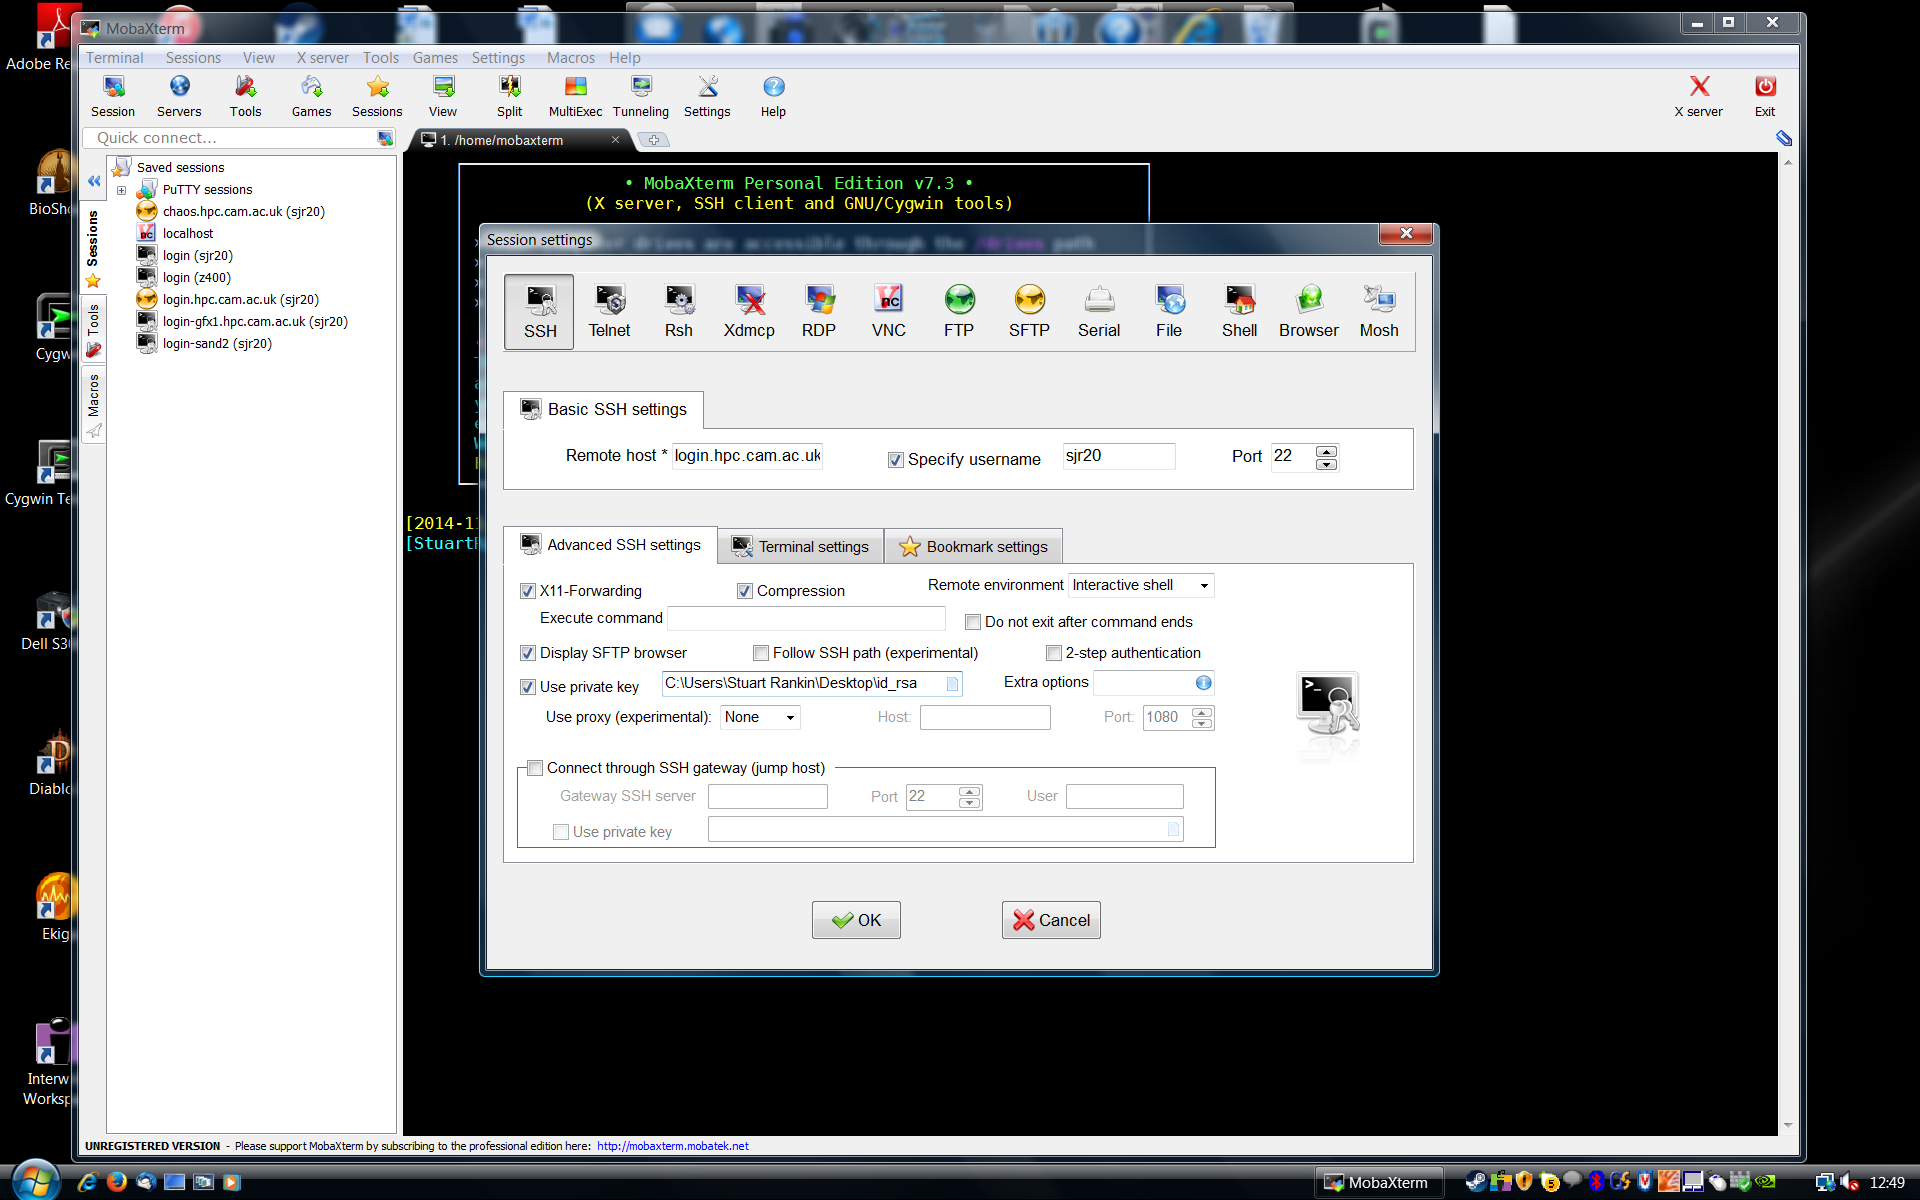
\includegraphics[height=0.8\textheight]{imgs/mobaxterm-SSH-settings2.png}}
\end{center}
\end{frame}

\begin{frame}{MobaXterm SSH (Windows)}
\begin{center}
\centerline{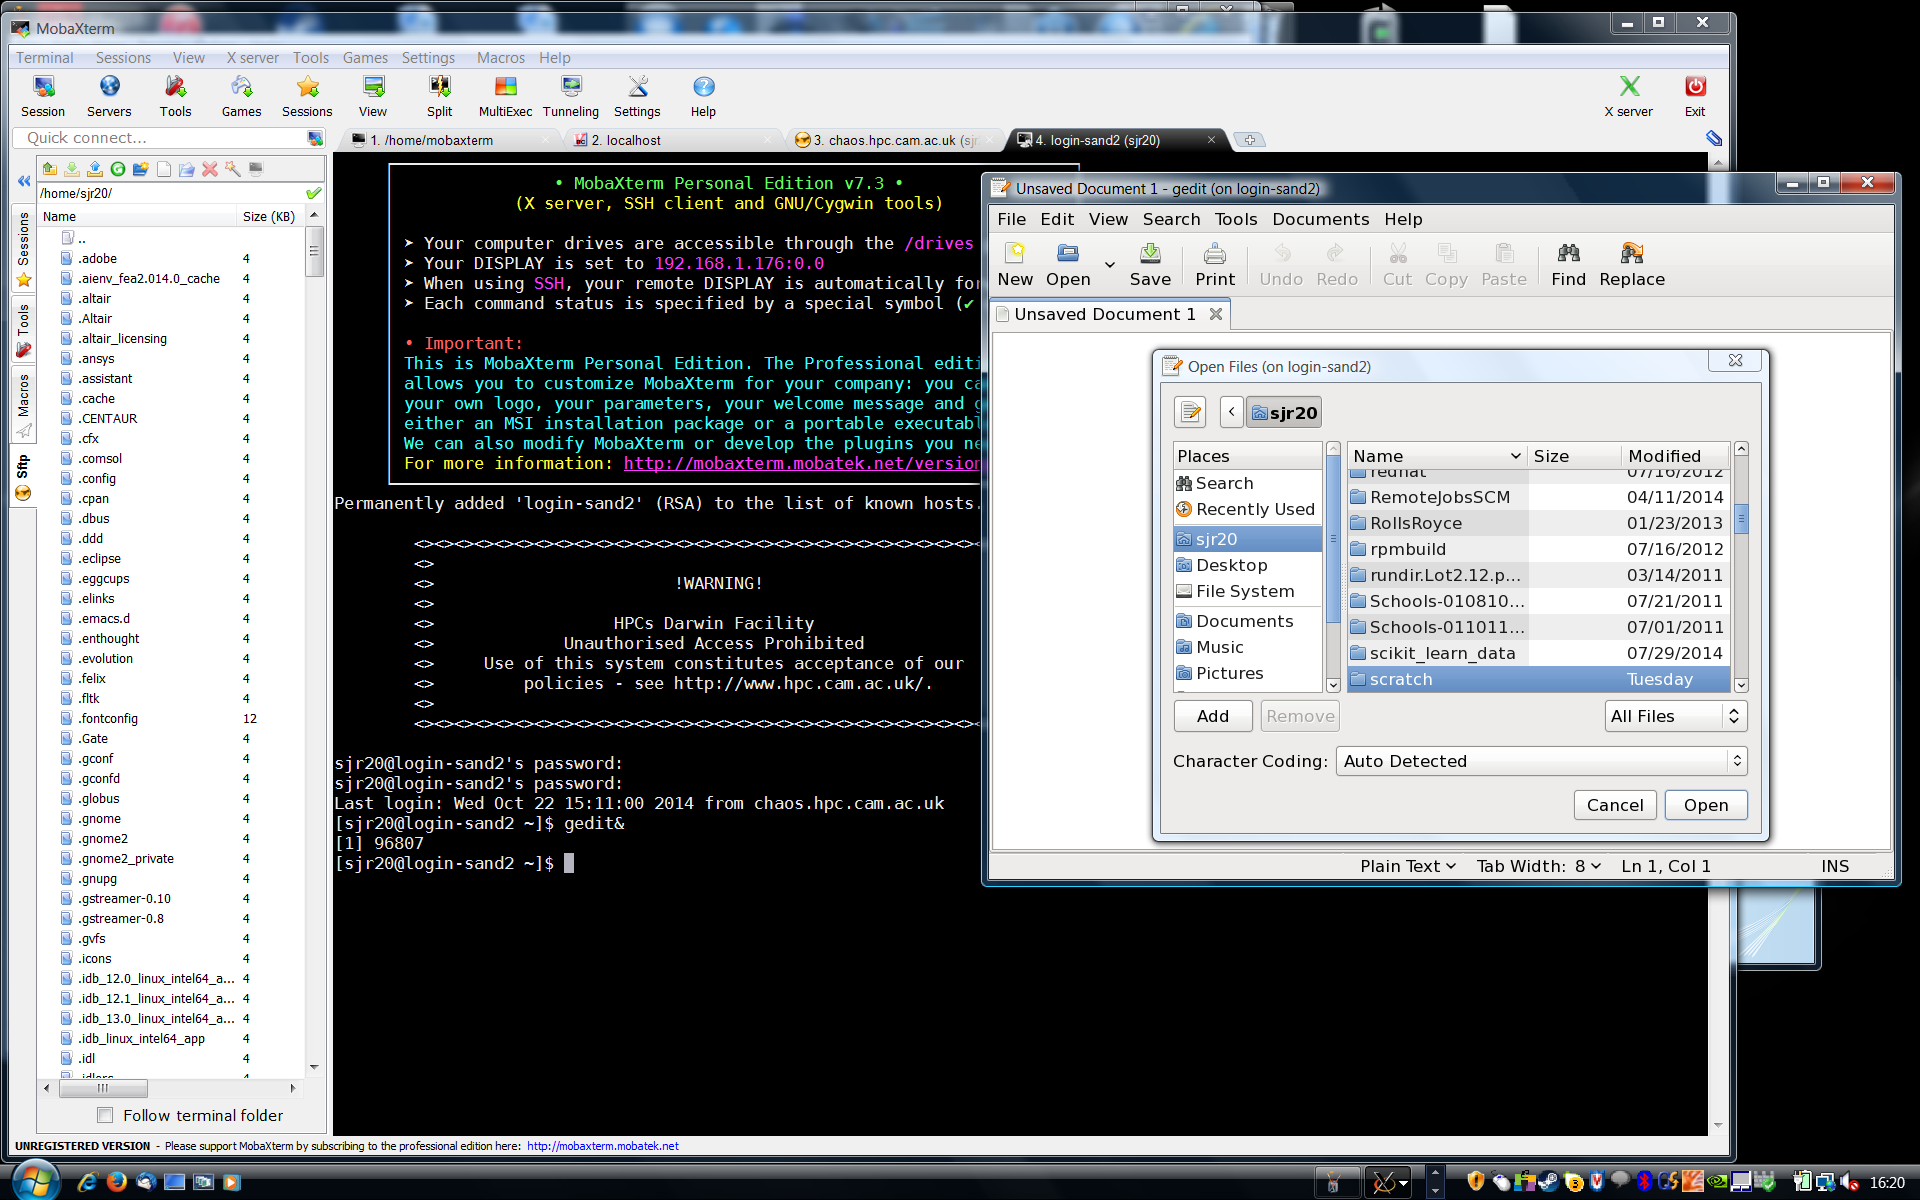
\includegraphics[height=0.8\textheight]{imgs/mobaxterm-SSH-session.png}}
\end{center}
\end{frame}

\section{Simple command line operations}
\begin{frame}{Simple command line operations}
\begin{itemize}
\item{Some simple exercises will help us gauge your experience.}
\item{Exercise 1: Login with SSH.}
\item{Exercise 2: SFTP file transfer.}
\item{Exercise 3: Navigating the command line.}
\end{itemize}
\end{frame}

\subsection{Exercise 1: Login with SSH}
\begin{frame}{Exercise 1: Login}
Using a Linux terminal you will login to the cluster with your HPC training account.
\begin{itemize}
\item{Start the terminal by double clicking on the terminal icon}
\item In your terminal enter:
\item{ssh -Y \textbf{abc123}@login-cpu.hpc.cam.ac.uk}\\
Replace abc123 with your training account username 
\item {Enter your password as supplied on the sheet}
\item{Leave this terminal open, you will need it for exercise 2!}
\end{itemize}
\end{frame}

\subsection{Exercise 2: SFTP file transfer - pt1}
\begin{frame}{Exercise 2: Transfer some files}
You will need to transfer the exercise files to the cluster.
\begin{itemize}
\item{Open a second Linux terminal on your training computer.}
\item{Enter this command: cd \alert{\footnotesize \path{~\Course_material}}}
\item{Check the file 'exercises.tar is in your directory listing}
\item{Hint: ls}
\end{itemize}
\end{frame}

\subsection{Exercise 2: SFTP file transfer - pt2}
\begin{frame}{Exercise 3: Transfer some files}
Transfer the exercises.tar to your HPC home folder.
\begin{itemize}
\item \alert{\footnotesize sftp abc123@login.hpc.cam.ac.uk}\\
Change abc123 to your training account username
\item{The command: \alert{\footnotesize put exercises.tar} will transfer the file from your local computer to the remote one}
\end{itemize}
\end{frame}

\subsection{Excercise 3: Unzip the excercises.tar file}
\begin{frame}{Exercise 3: Unzip the excercises.tar file}
  \begin{itemize}

\item[(a)]{Use the \alert{cd} command to enter the $\tilde{}$/hpc-work directory and then list the contents --- you should see the copy of exercises.tgz.}
 \visible<3->{\begin{description}
\item[\emph{Hints:}]{Do \alert{cd\quad$\tilde{}$/hpc-work/} then \alert{ls -al}. Note that \alert{cd ..} will take you back up one step to the home directory.}
\end{description}}

\item{Unpack the tar archive to create an exercise subdirectory.}
\visible<4->{\begin{description}
\item[\emph{Hints:}]{Do \alert{tar -zxvf exercises.tar}}
\end{description}}
\end{itemize}
\end{frame}


\subsection{Excercise 4: Navigating the command line}
\begin{frame}{Exercise 4: File listings}
\begin{itemize}

\item[(a)]{In a terminal logged into the cluster list the contents of your current directory \alert{ls}. This won't show everything --- use \alert{ls -al} for a long listing showing all files. Initially you will start in your home directory --- use \alert{pwd} to print the name of your current working directory. If you get lost, you can always do \alert{cd} without arguments to return to your home directory.}

\item[(b)]{Focus your long listing on \alert{all files with names beginning ``exercise''}.}
 \visible<2->{\begin{description}
\item[\emph{Hints:}]{Do \alert{ls -al exercise*}}
\end{description}}

\item[(c)]{Print a long listing of the subdirectory \alert{hpc-work}.}
 \visible<3->{\begin{description}
\item[\emph{Hints:}]{Do \alert{ls -al hpc-work/}. Note that omitting the / reveals that the item hpc-work is actually a shortcut (technically a symbolic link) to \alert{/hpc-work/username}.}
 \end{description}}

\end{itemize}
\end{frame}

\subsection{Excercise 5: Learn more about a command}
\begin{frame}{Exercise 5: Learn more about a command}
\begin{itemize}
    
\item[(a)]{View the man page for the \alert{cp} command by doing \alert{man cp}. Use \alert{SPACE} to page down and \alert{b} to page up. Press \alert{q} to exit the manual page command.}

\item[(b)]{Copy \alert{exercises.tar} to the $\tilde{}$/hpc-work directory. Note that $\tilde{}$ is just a convenient shorthand for your home directory. Omitting the $\tilde{}$/ will look for a hpc-work in the current directory.}
\visible<2->{\begin{description}
\item[\emph{Hints:}]{Do \alert{cp exercises.tsr\quad$\tilde{}$/hpc-work/}. Note that you can often reduce typing by pressing \alert{TAB}.}
\end{description}}
\end{itemize}
 \end{frame}







\subsection{Remote Desktop}
\begin{frame}[fragile]{Connecting: Remote Desktop}
\begin{itemize}
\item First time starting a remote desktop:
\begin{semiverbatim}
\footnotesize
[sjr20@login-a-1 ~]\$ vncserver

You will require a password to access your desktops.

Password: 
Verify:   
Would you like to enter a view-only password (y/n)? n

New 'login-a-1:99 (sjr20)' desktop is login-a-1:{\color{red}99}

Starting applications specified in /home/sjr20/.vnc/xstartup
Log file is /home/sjr20/.vnc/login-a-1:99.log
\end{semiverbatim}
\item{NB Choose a \alert{different} password for VNC.}
\item{The VNC password protects your desktop from other users.}
\item{Remember the unique display number ({\color{red}99} here) of your desktop.}
\end{itemize}
\end{frame}

\begin{frame}[fragile]{Connecting: Remote Desktop}
\begin{itemize}
\item Remote desktop already running:
\begin{semiverbatim}
\footnotesize
[sjr20@login-a-1 ~]\$ vncserver -list

TigerVNC server sessions:

X DISPLAY #     PROCESS ID
:99             130655
\end{semiverbatim}
\smallskip\item Kill it:
\begin{semiverbatim}
\footnotesize
[sjr20@login-a-1 ~]\$ vncserver -kill :99
Killing Xvnc process ID 130655
\end{semiverbatim}
\smallskip\item\alert{Typically you only need {\color{red}one} remote desktop.}
\item\alert{Keeps running until killed, or the node reboots.}
\end{itemize}
\end{frame}

%\begin{frame}{TurboVNC Session}
%\begin{center}
%\centerline{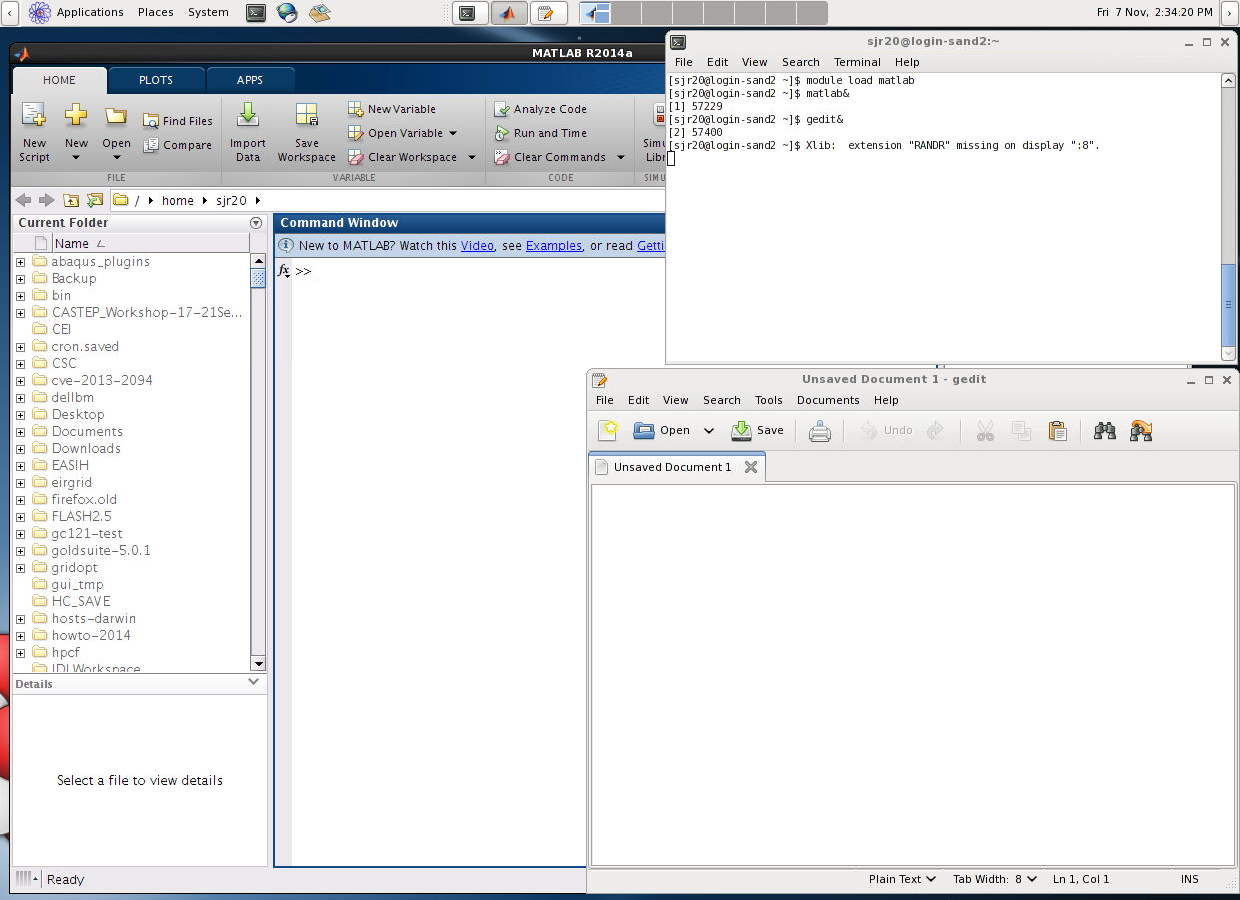
\includegraphics[width=0.85\textwidth]{imgs/linux-turbovnc.png}}
%\end{center}
%\end{frame}

%\begin{frame}{Linux TurboVNC Control Panel}
%\begin{center}
%\centerline{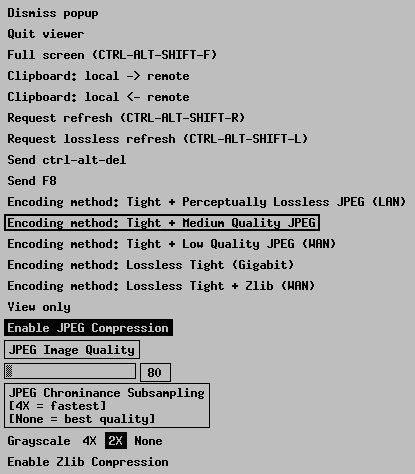
\includegraphics[height=0.8\textheight]{imgs/linux-turbovnc-F8.png}}
%\end{center}
%\end{frame}

\begin{frame}{Connecting: Remote Desktop (MobaXterm)}
\begin{center}
\centerline{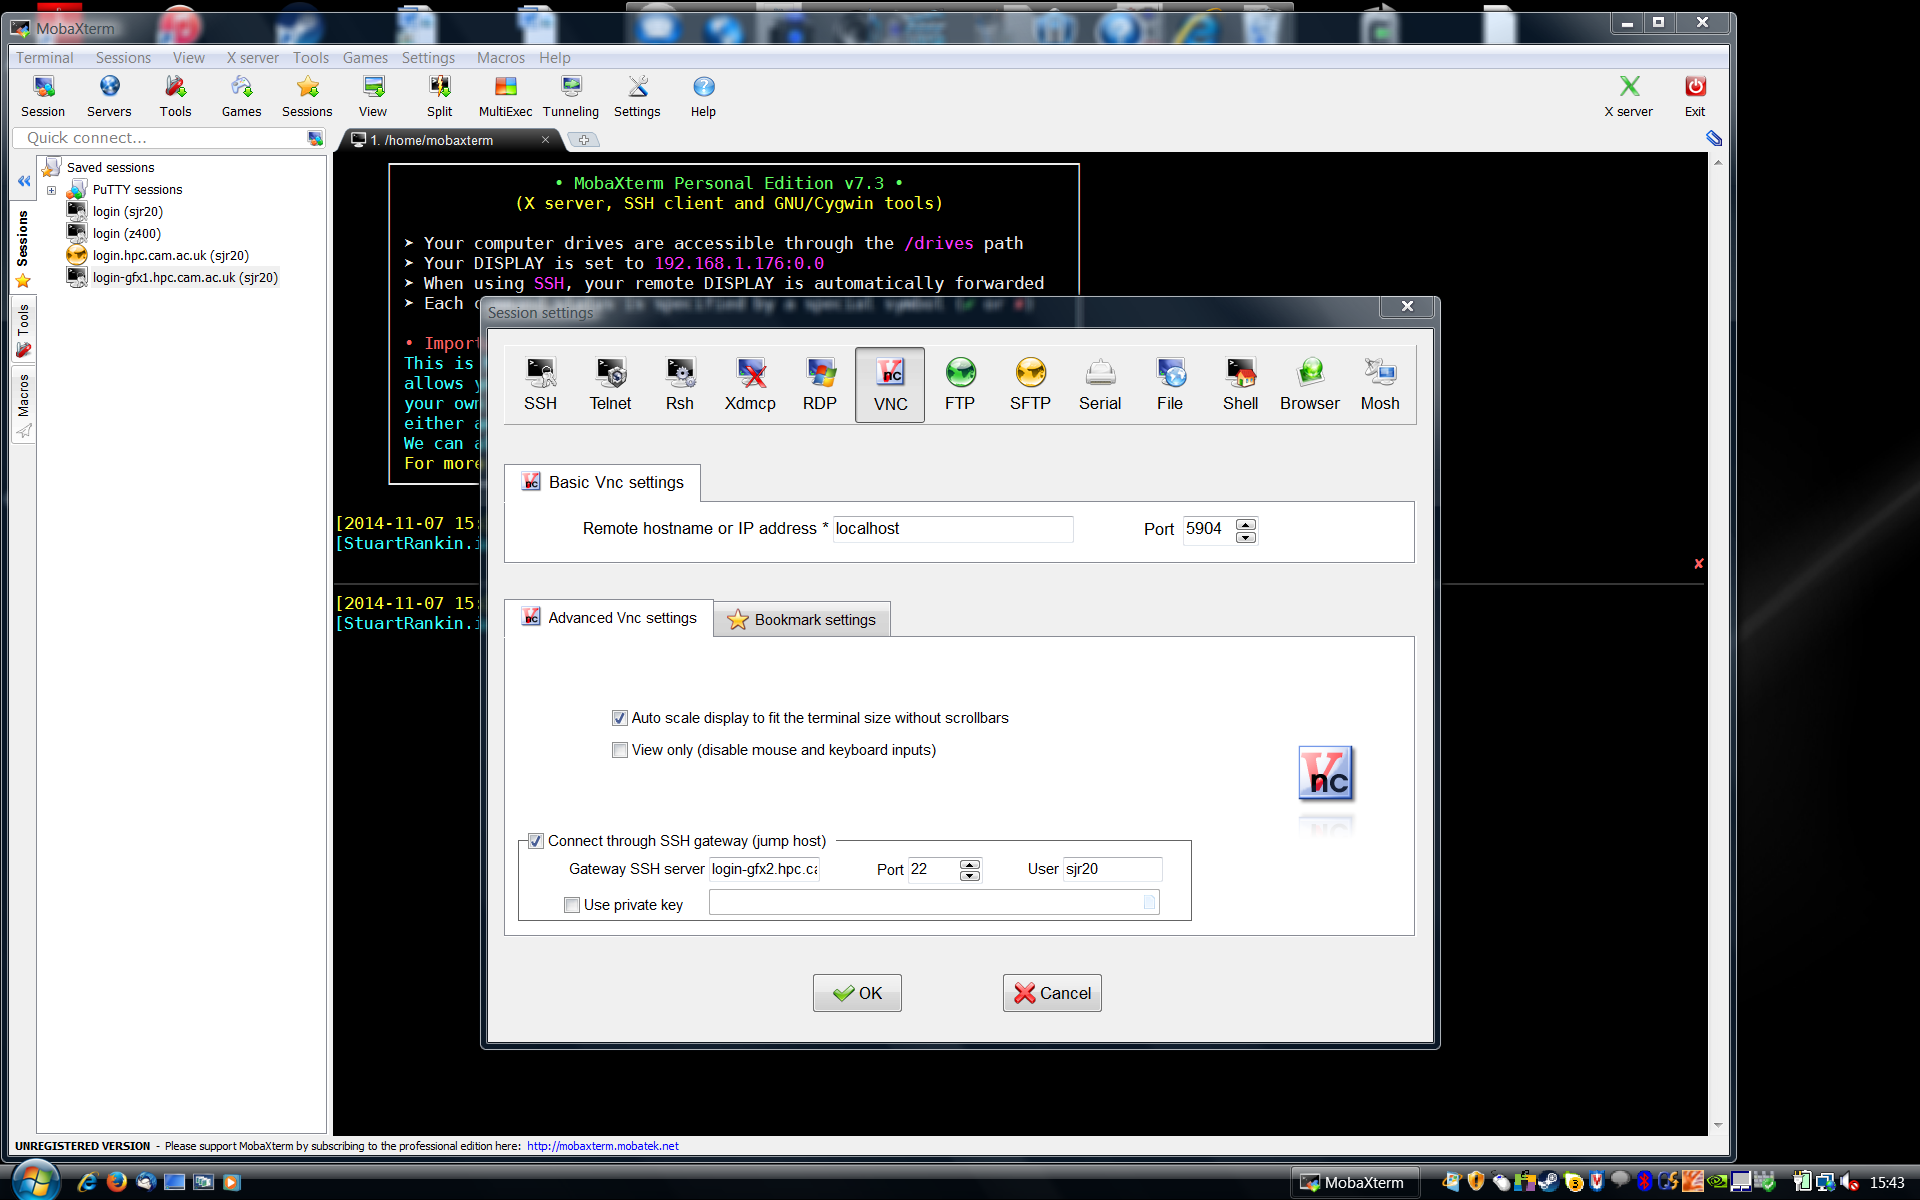
\includegraphics[height=0.8\textheight]{imgs/mobaxterm-turbovnc.png}}
\end{center}
\end{frame}
\part{Using HPC}
\begin{frame}
\partpage
\end{frame}

\section{User Environment}
\begin{frame}{Using HPC: User Environment}
\begin{itemize}
\item<1,3->{\visible<1>{CentOS Linux 7.4 (}\alert<1>{{\color<3->{red}Red Hat Enterprise Linux 7}\visible<1>{.4 rebuild)}}}
\begin{itemize}
\item{\visible<1>{bash shell}}
\item{\visible<1>{Gnome or XFCE4 desktop \alert{(if you want)}}}
\item{\visible<1>{GCC compilers and other development software.}}
\end{itemize}
\item<2->{But you don't need to know that.}
\end{itemize}
\end{frame}

\subsection{Filesystems}
\begin{frame}{User Environment: Filesystems}
When you apply for an HPC account a home directory is created for you. 
\begin{itemize}
\item{\alert{/home/<username>}}
\begin{itemize}
\item{40GB quota.}
\item{Visible equally from all nodes.}
\item{Single storage server.}
\item{Hourly, daily, weekly snapshots copied to tape.}
\item{Not intended for job outputs or large/many input files.}
\end{itemize}
\item{\alert{/rds/user/<username>hpc-work}}
\begin{itemize}
\item{Visible equally from all nodes.}
\item{Larger and faster (1TB initial quota).}
\item{Intended for job inputs and outputs.}
\item{{\color{red}Not backed up.}}
 \pause
\end{itemize}
\end{itemize}
\end{frame}

\subsection{Exceeding 1TB of HPC work}
\begin{frame}{Our storage services}
\begin{itemize}
\item{We have several storage services for users that need to exceed 1TB.}
\pause
\item{\alert{http://www.uis.cam.ac.uk/initiatives/storage-strategy/storage-services}}
\item{The most relevant services to HPC are RCS and RDS.}
\item{RCS - Research Cold Store is for data that isn't changing, data goes to disk then two sets of tapes.}
\item{RDS - Research Data Store, non backed up high performance storage for projects.}
\end{itemize}
\end{frame}

\subsection{Snapshots}
\begin{frame}{Filesystems: Snapshots}
\begin{itemize}
\item<1->{ZFS snapshots on /home are taken hourly, daily and weekly}
\item<2->{{\color{red}No backups are made of data in the RDS directories - take care when deleting.}}
\item<3->{Snapshots are not backups, they are retained for two weeks}
\item<4->{\color{red}Very short lived files are unlikely to get written to snapshots}
\item{The file needs exist long enough to get into a snapshot.}
\item{It is possible to search /home/.zfs/snapshot and browse the snapshots}
\item {Locatre the most recent version of the file then copy it back to your home folder} 
\end{itemize}
\end{frame}

\begin{frame}[fragile]{Filesystems: Quotas}
\begin{itemize}
\item{quota}
\begin{semiverbatim}
\tiny
[ps459@login-e-13 hpc-work]\$ quota
Filesystem  GiBytes    quota   limit   grace    files    quota    limit   grace User/group
/home          12.4     40.0    40.0       0    ----- No ZFS File Quotas  ----- U:ps459
/rds-d1        89.2   1024.0  1126.4       -   757345  1048576  1048576       - G:ps459
/rds-d1        22.1   1024.0  1024.0       -   113475  1048576  1048576       - G:rds-ps459-test
\end{semiverbatim}
\item<1-|handout:1->{\alert{Aim to stay below the soft limit (\emph{quota}).}}
\item<2-|handout:1->{\alert{Once over the soft limit, you have 7 days grace to return below.}}
\item<3-|handout:2>{\alert{When the grace period expires, or you reach the hard limit (\emph{limit}), no more data can be written.}}
\item<4-|handout:2>{\alert{It is important to rectify an out of quota condition ASAP.}}
\end{itemize}
\end{frame}

\begin{frame}{Filesystems: Permissions}
\begin{itemize}
\item{\color{red}Be careful and if unsure, please ask support.}
\begin{itemize}
\item{Can lead to \alert{accidental destruction} of your data or \alert{account compromise}.}
\end{itemize}
\item{Avoid changing the permissions on your home directory.}
\begin{itemize}
\item{Files under /home are particularly security sensitive.}
\item{Easy to break passwordless communication between nodes.}
\end{itemize}
\end{itemize}
\end{frame}

\section{Software}
\begin{frame}{Using HPC: Software}
\begin{itemize}
\item{Free software accompanying \alert{Red Hat Enterprise} is (or can be) provided.}
\item{Other software (free and non-free) is available via \alert{modules}.}
\item{Some proprietary software may not be generally accessible.}
\item{See \alert{http://www.hpc.cam.ac.uk/using-clusters/software}.}
\item{New software may be possible to provide on request.}
\item{\alert{Self-installed software must be properly licensed.}}
  \pause
\item{\color{red}\emph{sudo will not work.}\/ (You should be worried if it did.)}
\end{itemize}
\end{frame}

\subsection{Environment Modules}
\begin{frame}[fragile]{User Environment: Environment Modules}
\begin{itemize}
\item{Modules load or unload additional software packages.}
\item{Some are \alert{required} and automatically loaded on login.}
\item{Others are optional extras, or possible replacements for other modules.}
\item{\alert{Beware} unloading default modules in $\tilde{}\text{/.bashrc}$.}
\item{\alert{Beware} overwriting environment variables such as PATH and LD\_LIBRARY\_PATH in $\tilde{}\text{/.bashrc}$. If necessary append or prepend.}
\end{itemize}
\end{frame}

\subsection{Environment Modules}
\begin{frame}[fragile]{User Environment: Environment Modules}
\begin{itemize}
\item{Currently loaded:}
\begin{semiverbatim}
\scriptsize
module list
Currently Loaded Modulefiles:
 1) dot                            2) singularity/current            2) intel/impi/2017.4/intel       4) intel/libs/daal/2017.4
....plus several more default modules
\end{semiverbatim}
\medskip
\item{Available:}
\begin{semiverbatim}
\scriptsize
module av
\end{semiverbatim}
\end{itemize}
\end{frame}

\begin{frame}[fragile]{User Environment: Environment Modules}
\begin{itemize}
\item{Whatis:}
\begin{semiverbatim}
\tiny
module whatis openmpi-3.0.0-gcc-4.8.5-n2hvjgm
openmpi-3.0.0-gcc-4.8.5-n2hvjgm: The Open MPI Project is an open source...
\end{semiverbatim}
\medskip
\item{Load:}
\begin{semiverbatim}
\scriptsize
module load openmpi-3.0.0-gcc-5.4.0-4ryklvu
\end{semiverbatim}
\medskip
\item{Unload:}
\begin{semiverbatim}
\scriptsize
module unload openmpi-3.0.0-gcc-5.4.0-4ryklvu
\end{semiverbatim}
\end{itemize}
\end{frame}

\begin{frame}[fragile]{User Environment: Environment Modules}
\begin{itemize}
\item{Matlab}
\begin{semiverbatim}
\scriptsize
module load matlab/r2017b
\end{semiverbatim}
\medskip\pause
\item{Invoking matlab in batch mode:\hfill\\
  \qquad \alert{matlab -nodisplay -nojvm -nosplash command}\hfill\\
  where the file \alert{command.m} contains your matlab code.}
  \pause
  \item{The current site license contains the Parallel Computing Toolbox.}
\end{itemize}
\end{frame}

\begin{frame}[fragile]{User Environment: Environment Modules}
\begin{itemize}
\item{Purge and Load Defaults:}
\begin{semiverbatim}
\scriptsize
module purge
\item{module load rhel7/default-peta4}
\end{semiverbatim}
\smallskip
\end{itemize}
\end{frame}

\subsection{Compilers}
\begin{frame}[fragile]{User Environment: Compilers}
  \begin{itemize}
    \item{Load a newer GCC}
\begin{semiverbatim}
\scriptsize
module show gcc-7.2.0-gcc-4.8.5-pqn7o2k
module load gcc-7.2.0-gcc-4.8.5-pqn7o2k
Your commands to compile your software....
\end{semiverbatim}
\medskip
\item{If you have compiled software yourself your run time environment must match compile time environment!}

\begin{semiverbatim}
\scriptsize
gcc -O3 -mtune=native code.c -o prog
gfortran -O3 -mtune=native code.f90 -o prog
\medskip
module load openmpi-3.0.0-gcc-4.8.5-n2hvjgm
mpicc -O3 -mtune=native mpi_code.c -o mpi_prog
mpif90 -O3 -mtune=native mpi_code.f90 -o mpi_prog
\end{semiverbatim}
\pause
\end{itemize}
\end{frame}

\section{Excercises}

\subsection{Modules: Excercise 3}
\begin{frame}[fragile]{Excercise 3: Environment Modules}
\begin{itemize}
\item{Connect to the cluster using your training account: See excercise 1 if you have closed your terminal. }
\item{Get a list of modules that are currently loaded}
\item[\emph{Hints:}]{\alert{module list}}
\item{Get a list of available R modules}
\item[\emph{Hints:}]{\alert{module av R}}
\end{itemize}
\end{frame}

\subsection{Modules: Excercise 4}
\begin{frame}[fragile]{Excercise 5: Run an Rscript}
\begin{itemize}
\item{Connect to the cluster using your training account: See excercise 1 if you have closed your terminal.}
\item{In the exercises folder there is a file called test.r}
\item{Run this script using: Rscript hello.r }
\item{Load the module for: R/3.3.2}
\item[\emph{Hints:}]{\alert{module load R/3.3.2}}
\item{Run the script again: Rscript hello.r}
\end{itemize}
\end{frame}

\subsection{Local R library: Excercise 5}
\begin{frame}[fragile]{Exercise 5: Install the R library locally}
As a user you can create a local R library directory for packages that you want to install. 

\begin{itemize}
\item Load an R module: 
module load r-3.4.3-gcc-5.4.0-rbvhnga
\item Create a folder in your home for your own R package installs:
mkdir ~/my-R-libs
\item Make R aware of the new library location:
\begin{verbatim}
echo "R_LIBS_USER=~/my-R-libs" \textgreater .Renviron
\end{verbatim}
\item Start R:
R
\item Display your library paths:
.libPaths()
\item Try loading a library:
require(pander)
\item Its not insalled, lets install it:
install.packages("pander")
\item Try loading a library:
require(pander)
\item Library is now installed, lets quit R:
quit()
\end{itemize}
\end{frame}

\subsection{Excercise 5: explained}
\begin{frame}[fragile]{Excercise explained}
As a user you can create a local R library directory for packages that you want to install.
\begin{itemize}
\item First we load an R module, note the lower case r: module load r/(version). The lower case r is neccasary as upper case R modules are compiled for an older version of linux.
\item We create a folder for your local R package installs. This could be in your home or on HPC work.
mkdir ~/my-R-libs
\item In the root of your home directory we create a file .Renviron. This file is read by R and sets a variable which makes it aware of our local R library directory.
\item echo " " outputs the text between the quotes, \textgreater redirects the text into .Renviron which a file.
\item When we start R the .Renviron file is read and R will look for and install local packages in the local library directory.
\item .libPaths() is used to displays the R library locations where R modules will get installed. 
\item We then installing a package to the library using the R console:
\begin{verbatim}
install.packages("new_package_installation", "options", dependences=)
\end{verbatim}
Note that its possible to specify options or name other packages that are a dependency. 
\item Now you can load the library from the R terminal or inside an Rscript:
require(pander)
\end{itemize}
\end{frame}

\part{HPC Job Submission}
\begin{frame}
\partpage
\end{frame}

\section{Job Submission}
\begin{frame}{Using HPC: Job Submission}
\centerline{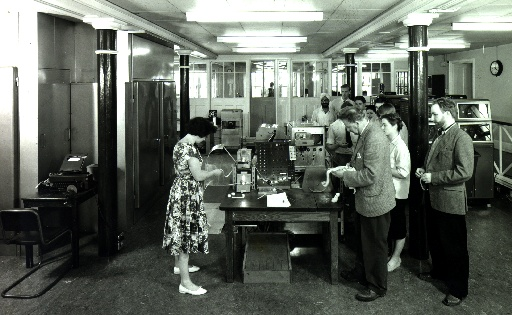
\includegraphics[width=1\textwidth]{imgs/EDSAC_2_1960.jpg}}
\end{frame}
\begin{frame}{Using HPC: Job Submission}
\begin{itemize}
\item{Compute resources are managed by a scheduler:\hfill\\\qquad\alert{SLURM}/PBS/SGE/LSF/\ldots}
\item{Jobs are submitted to the scheduler\hfill\\\qquad --- analogous to submitting jobs to a print queue\hfill\\\qquad --- a file (\emph{submission script}) is copied and queued\hfill\\\qquad \hphantom{---} for processing.}
\end{itemize}
\end{frame}

\begin{frame}{Using HPC: Job Submission}
\begin{itemize}
\item{Jobs are submitted from the \alert{login node}\hfill\\\qquad  --- not itself managed by the scheduler.}
\item{Jobs may be either non-interactive (\alert{batch}) or \alert{interactive}.}
\pause
\item{\alert{Batch} jobs run a shell script on the first of a list of allocated nodes.}
\item{\alert{Interactive} jobs provide a command line on the first of a list of allocated nodes.}
\end{itemize}
\end{frame}

\begin{frame}{Using HPC: Job Submission}
\begin{itemize}
\item{Jobs may use \alert{part} or \alert{all} of one or more nodes\hfill\\
\qquad --- the owner can specify \mbox{\tt --exclusive} to force exclusive\hfill\\\qquad\hphantom{---} node access.}
\item{Template submission scripts are available under\hfill\\
\qquad \alert{/usr/local/Cluster-Docs/SLURM}.}
\end{itemize}
\end{frame}

\begin{frame}[fragile]{Job Submission: Using SLURM}
\begin{itemize}
\item{Prepare a shell script and submit it to SLURM:}
\begin{semiverbatim}
\scriptsize
[abc123@login-a-1]\$ sbatch slurm_submission_script
Submitted batch job {\color{red}790299}
\end{semiverbatim}
\end{itemize}
\end{frame}

\begin{frame}[fragile]{Job Submission: Show Queue}
\begin{itemize}
\item{Submitted job scripts are copied and stored in a queue:}
\begin{semiverbatim}
\tiny
[abc123@login-a-1]\$ squeue -u abc123
             JOBID PARTITION     NAME     USER ST       TIME  NODES NODELIST(REASON)
            {\color{red}790299}   skylake     Test3  abc123 PD       0:00      2 (\only<1>{{\color{blue}Priority}}\only<2>{{\color{green}Resources}}\only<3>{{\color{red}AssocGrpCPUMinsLimit}})
            790290   skylake     Test2  abc123  R   27:56:10      2 cpu-a-[1,10]
\end{semiverbatim}
\end{itemize}
\end{frame}

\begin{frame}[fragile]{Job Submission: Monitor Job}
\begin{itemize}
\item{Examine a particular job:}
\begin{semiverbatim}
\scriptsize
[abc123@login-a-1]\$ scontrol show job={\color{red}790290}
\end{semiverbatim}
\end{itemize}
\end{frame}

\begin{frame}[fragile]{Job Submission: Cancel Job}
\begin{itemize}
\item{Cancel a particular job:}
\begin{semiverbatim}
\scriptsize
[abc123@login-a-1]\$ scancel {\color{red}790290}
\end{semiverbatim}
\end{itemize}
\end{frame}

\begin{frame}[fragile]{Job Submission: Scripts}
\begin{itemize}
\item{SLURM\hfill\\
In \alert{$\tilde{}$/job\_templates}, see examples: \alert{slurm\_submit.skylake.generic}, \alert{slurm\_submit.skylake.matlab}.}
  
\begin{semiverbatim}
\tiny
#!/bin/bash
#! Name of the job:
{\color<2->{red}#SBATCH} -J myjob
#! Which project should be charged:
{\color<2->{red}#SBATCH} -A TRAINING-CPU
#! How many whole nodes should be allocated?
{\color<2->{red}#SBATCH} --nodes=1
#! How many tasks will there be in total? (<= nodes*32)
{\color<2->{red}#SBATCH} --ntasks={\color<3->[rgb]{1,0,0}\only<1-3>{1}\only<4->{16}}
#! How much wallclock time will be required?
{\color<2->{red}#SBATCH} --time=02:00:00
#! Select partition:
{\color<2->{red}#SBATCH} -p skylake
...
\end{semiverbatim}
\item<2->{{\color{red}\#SBATCH} lines are \emph{structured comments}\hfill\\
\qquad --- correspond to sbatch command line options.}
\item<3->{\alert{The above job will be given {\color<3->[rgb]{1,0,0}\only<1-3>{1 cpu}\only<4->{16 cpus}} on 1 node for 2 hours (by default there is 1 task per node, and 1 cpu per task).}}
\end{itemize}
\end{frame}

\begin{frame}[fragile]{Job Submission: Accounting Commands}
\begin{itemize}
\item{How many core hours available do I have?}
\begin{semiverbatim}
\tiny
mybalance

User           Usage |        Account     Usage | Account Limit Available (hours)
---------- --------- + -------------- --------- + ------------- ---------
sjr20              3 |    SUPPORT-CPU     2,929 |    22,425,600 {\color{red}22,422,671}
sjr20              0 |    SUPPORT-GPU         0 |        87,600    {\color{red}87,600}
\end{semiverbatim}
\smallskip
\item{How many core hours does some other project or user have?}
\begin{semiverbatim}
\tiny
gbalance -p SUPPORT-CPU

User           Usage |        Account     Usage | Account Limit Available (hours)
---------- --------- + -------------- --------- + ------------- ---------

pfb29          2,925 |    SUPPORT-CPU     2,929 |    22,425,600 22,422,671
sjr20 *            3 |    SUPPORT-CPU     2,929 |    22,425,600 22,422,671
...
(Use -u for user.)
\end{semiverbatim}
\smallskip
\item{List all jobs charged to a project/user between certain times:}
\begin{semiverbatim}
\Tiny
gstatement -p SKYLAKE  -u xyz10 -s "2018-04-01-00:00:00" -e "2018-04-30-00:00:00" 
       JobID      User    Account    JobName  Partition                 End ExitCode      State  CompHrs 
------------ --------- ---------- ---------- ---------- ------------------- -------- ---------- -------- 
263              xyz10 support-c+ _interact+    skylake 2018-04-18T19:44:40      0:0    TIMEOUT      1.0
264              xyz10 support-c+ _interact+    skylake 2018-04-18T19:48:07      0:0 CANCELLED+      0.1
275              xyz10 support-c+ _interact+    skylake             Unknown      0:0    RUNNING      0.3
...
\end{semiverbatim}
\end{itemize}
\end{frame}

\subsection{Single Node Jobs}
\begin{frame}[fragile]{Job Submission: Single Node Jobs}
\begin{itemize}
\item{Serial jobs requiring large memory, or OpenMP codes.}
\begin{semiverbatim}
\scriptsize
#!/bin/bash
\ldots
#SBATCH --nodes=1
\uncover<2-|handout:2->{{\color{red}#SBATCH --ntasks=1
# Default is 1 task per node}} 
\uncover<3-|handout:2->{{\color{red}#SBATCH --cpus-per-task=\only<3-5|handout:2>{1}\only<6,8-|handout:3,5->{32 # Whole node}\only<7|handout:4>{16  # Half node}
\only<3-5|handout:2>{# Default is 1 cpu (core) per task}}}
\uncover<4-5|handout:2>{{\color{red}#SBATCH --mem=5990
# Memory per node in MB - default is pro rata by cpu number}}
\uncover<5|handout:2>{{\color{red}# Increasing --mem or --cpus-per-task implicitly increases the other}}
\ldots
\uncover<6-|handout:3->{{\color{red}export OMP\_NUM\_THREADS=\only<6|handout:3>{32}\only<7-|handout:4->{16}  # For OpenMP across \only<6|handout:3>{32}\only<7-|handout:4->{16} cores\only<8-|handout:5->{ (using all memory)}}}
\$application \$options
\ldots
\end{semiverbatim}
\end{itemize}
\end{frame}

\subsection{MPI Jobs}
\begin{frame}[fragile]{Job Submission: MPI Jobs}
\begin{itemize}
\item{Parallel job across multiple nodes.}
\begin{semiverbatim}
\scriptsize
#!/bin/bash
\ldots
#SBATCH --nodes={\color{red}4}
#SBATCH --ntasks=\alert{\only<1|handout:1>{128}\only<2-|handout:2->{64}}     # \only<1|handout:1>{i.e.\ {\color[rgb]{0,0.8,0}32}}\only<2-|handout:2->{i.e.\ {\color[rgb]{0,0.8,0} 16}}x{\color{red}4} MPI tasks in total.
\uncover<2-|handout:2->{{\color{red}#SBATCH --cpus-per-task=2}}
\ldots
mpirun\only<2-|handout:2->{ -ppn {\color[rgb]{0,0.8,0}16}} -np \alert{\only<1|handout:1>{128}\only<2-|handout:2->{64}} \$application \$options
\ldots
\end{semiverbatim}
\item<3-|handout:2->{\small SLURM-aware MPI launches remote tasks via SLURM.}
\item<3-|handout:2->{\small The template script uses \$SLURM\_TASKS\_PER\_NODE to set PPN.}
\end{itemize}
\end{frame}

\subsection{Hybrid Jobs}
\begin{frame}[fragile]{Job Submission: Hybrid Jobs}
\begin{itemize}
\item{Parallel jobs using both MPI and OpenMP.}
\begin{semiverbatim}
\scriptsize
#!/bin/bash
\ldots
#SBATCH --nodes={\color{red}4}
#SBATCH --ntasks=\alert{64}     # i.e.\ {\color[rgb]{0,0.8,0}16}x{\color{red}4} MPI tasks in total.
#SBATCH --cpus-per-task={\color{brown}2}
\ldots
{\color{brown}export OMP\_NUM\_THREADS=2   # i.e.\ 2 threads per MPI task.}
mpirun -ppn {\color[rgb]{0,0.8,0}16} -np \alert{64} \$application \$options
\ldots
\end{semiverbatim}
\item<2->{\small This job uses \alert{128 CPUs} (each MPI task splits into 2 OpenMP threads).}
\end{itemize}
\end{frame}

\subsection{High Throughput Jobs}
\begin{frame}[fragile]{Job Submission: High Throughput Jobs}
\begin{itemize}
\item{Multiple serial jobs across multiple nodes.}
\item{Use \alert{srun} to launch tasks (\alert{job steps}) within a job.}
\begin{semiverbatim}
\scriptsize
#!/bin/bash
\ldots
#SBATCH --nodes=2
\ldots
cd directory\_for\_job1
\alert{srun} {\color<3>{red}--exclusive} {\color<2>{red}-N 1 -n 1} \$application \$options\_for\_job1 > output 2> err {\color<4>{red}&}
cd directory\_for\_job2
\alert{srun} {\color<3>{red}--exclusive} {\color<2>{red}-N 1 -n 1} \$application \$options\_for\_job2 > output 2> err {\color<4>{red}&}
...
cd directory\_for\_job64
\alert{srun} {\color<3>{red}--exclusive} {\color<2>{red}-N 1 -n 1} \$application \$options\_for\_job64 > output 2> err {\color<4>{red}&}
{\color<5>{red}wait}
\end{semiverbatim}
\end{itemize}
\end{frame}

\section{Exercise 11: High Throughput Jobs}
\begin{frame}{Exercise 11: Submitting a Matlab job}
\begin{itemize}
\item{Submit a job which will run \alert{matlab} on the \alert{file.m} command file (which contains just the \alert{ver} command).}
\visible<2->{\begin{description}
\item[\emph{Hints:}]{\scriptsize\begin{enumerate}
\item{Load the matlab module using the \alert{job\_script} in your exercises directory.}
\item{Set the value of application to\hfill\break{}\alert{\"{}matlab -nodesktop -nosplash -nojvm\"{}}}
\item{Set the value of options to \alert{\"{}-r file\"{}}}
\item{Submit the job with \alert{sbatch job\_script}. The jobid is then printed.}
\item{Watch the job in the queue with \alert{squeue}.}
\item{After it has disappeared, open the output file \alert{slurm-jobid.out} in your editor. It should contain a list of licensed Matlab features.}
  \item{For more demanding work you can increase the available memory by increasing the number of cpus.}
  \end{enumerate}%
}
\end{description}}
\end{itemize}
\end{frame}

\subsection{Exercise 12: High Throughput Jobs}
\begin{frame}{Exercise 12: Submitting compiled code}
\begin{itemize}
\item{Submit a job which will run a copy of your hello program on 1 cpu.}
\visible<2->{\begin{description}
\item[\emph{Hints:}]{\scriptsize\begin{enumerate}
\item{Edit the script \alert{job\_script} in your exercises directory. Set:\hfill\\
\alert{\#SBATCH --nodes=1}\hfill\\
\alert{\#SBATCH --ntasks=1}\hfill\\
\alert{application="./hello"}}
\item{Submit the job with \alert{sbatch job\_script}. The jobid is then printed.}
\item{Watch the job in the queue with \alert{squeue}.}
\item{After it has disappeared, open the output file \alert{slurm-jobid.out} in your editor. There should be exactly one ``Hello, World!'' message.}
\end{enumerate}%
}
\end{description}}
\end{itemize}
\end{frame}

\subsection{Interactive Jobs}
\begin{frame}[fragile]{Job Submission: Interactive}
\begin{itemize}
\item{Compute nodes are accessible via SSH \alert{while you have a job running on them}.}
\pause
\item{Alternatively, submit an interactive job:}
\begin{semiverbatim}
\alert{sintr -A TRAINING-CPU -N1 -n8 -t 2:0:0}
\end{semiverbatim}
\medskip
\pause
\item{Within the window (screen session):}
\begin{itemize}
\item[$\ast$]{Launches a shell on the first node (when the job starts).}
\item[$\ast$]{Graphical applications should display correctly.}
\item[$\ast$]{Create new shells with \alert{ctrl-a c}, navigate with \alert{ctrl-a n} and \alert{ctrl-a p}.}
\item[$\ast$]{\alert{ssh} or \alert{srun} can be used to start processes on any nodes in the job.}
\item[$\ast$]{SLURM-aware MPI will do this automatically.}
\end{itemize}
\end{itemize}
\end{frame}

\section{Array Jobs}
\subsection{Array Jobs}
\begin{frame}[fragile]{Job Submission: Array Jobs}
\begin{itemize}
\item{\alert{$http://slurm.schedmd.com/job\_array.html$}}
\item{Used for submitting and managing large sets of similar jobs.}
\item{Each job in the array has the same \alert{initial} options.}
\item{SLURM}
\begin{semiverbatim}
\scriptsize
[abc123@login-a-1]\$ sbatch --array=\only<1,2>{{\color{red}1-7}}\only<2>{{\color{red}:2}}\only<3->{{\color{red}1,3,5,7}} -A TRAINING-CPU submit\_script
Submitted batch job {\color[rgb]{0,0.6,0}791609}
\tiny
\uncover<4->{[abc123@login-a-1]\$ squeue -u abc123
             JOBID PARTITION     NAME     USER ST       TIME  NODES NODELIST(REASON)
          {\color[rgb]{0,0.6,0}791609}\_{\color{red}1} skylake      hpl    abc123  R       0:06      1 cpu-a-6
          {\color[rgb]{0,0.6,0}791609}\_{\color{red}3} skylake      hpl    abc123  R       0:06      1 cpu-a-16
          {\color[rgb]{0,0.6,0}791609}\_{\color{red}5} skylake      hpl    abc123  R       0:06      1 cpu-a-7
          {\color[rgb]{0,0.6,0}791609}\_{\color{red}7} skylake      hpl    abc123  R       0:06      1 cpu-a-7
}
\end{semiverbatim}
\uncover<5->{\centerline{{\color[rgb]{0,0.6,0}791609}\_{\color{red}1}, {\color[rgb]{0,0.6,0}791609}\_{\color{red}3}, {\color[rgb]{0,0.6,0}791609}\_{\color{red}5}, {\color[rgb]{0,0.6,0}791609}\_{\color{red}7}}}
\smallskip
\uncover<6->{\centerline{i.e.\ \$\{{\color[rgb]{0,0.6,0}SLURM\_ARRAY\_JOB\_ID}\}\_\$\{{\color{red}SLURM\_ARRAY\_TASK\_ID}\}}}
\smallskip
\uncover<7->{\leftline{\small SLURM\_ARRAY\_JOB\_ID${}={}$SLURM\_JOBID for the first element.}}
\end{itemize}
\end{frame}

\begin{frame}[fragile]{Job Submission: Array Jobs (ctd)}
\begin{itemize}
\item{Updates can be applied to specific array elements using \$\{{\color[rgb]{0,0.6,0}SLURM\_ARRAY\_JOB\_ID}\}\_\$\{{\color{red}SLURM\_ARRAY\_TASK\_ID}\}}
\item{Alternatively operate on the entire array via \$\{{\color[rgb]{0,0.6,0}SLURM\_ARRAY\_JOB\_ID}\}}.
\item{Some commands still require the SLURM\_JOB\_ID (sacct, sreport, sshare, sstat and a few others).}
\pause
\item{Exercise 7 - Array Jobs.}
\end{itemize}
\end{frame}

\section{Excercise 13: Array Jobs}
\begin{frame}{Exercise 13: Array Jobs}
\begin{itemize}
\item{Submit your last job in the form of an array with indices 1-32. Use -H with sbatch to mark the array as held (so that it won't run immediately).}
\visible<2->{\begin{description}
\item[\emph{Hints:}]{\scriptsize\begin{enumerate}
\item{Use \alert{sbatch -H -{}-array=1-32 job\_script}}
\item{Use \alert{squeue -u userid} to see your array job. Note that \alert{-r} reports each array element individually.}
\end{enumerate}%
}
\end{description}}
\item{Release array element 1 and allow it to run. Then release the others.}
\visible<3->{\begin{description}
\item[\emph{Hints:}]{\scriptsize\begin{enumerate}
\item{Use \alert{scontrol release \$\{{SLURM\_ARRAY\_JOB\_ID}\}\_{{\color{red}1}}}}
\item{Use \alert{squeue -u userid} again to watch what happens.}
\item{Release the others with\hfill\break
\null\qquad scontrol release \$\{{SLURM\_ARRAY\_JOB\_ID}\}\hfill\break
i.e. use the array id to release the entire array.}
  \item{When all the jobs complete you should have 32 slurm-\$\{SLURM\_ARRAY\_JOB\_ID\}\_N.out files saying hello from various cpus on possibly multiple nodes.}
\end{enumerate}%
}
\end{description}}
\end{itemize}
\end{frame}

\subsection{Scheduling}
\begin{frame}{Scheduling}
\begin{itemize}
\item{SLURM scheduling is multifactor:}
  \pause
\begin{itemize}
\item{\alert{QoS} --- payer or non-payer?}
  \pause
\item{\alert{Age} --- how long has the job waited?\hfill\\\qquad
  \alert{Don't cancel jobs that seem to wait too long.}}
  \pause
\item{\alert{Fair Share} --- how much recent usage?\hfill\\\qquad
  \alert{Payers with little recent usage receive boost (not implemented yet).}}
  \pause
\item{\alert{sprio -j jobid}}
\end{itemize}
\pause
\item{\alert{Backfilling}}
\begin{itemize}
  \item{Promote lower priority jobs into gaps left by higher priority jobs.}
    \item{Demands that the higher priority jobs not be delayed.}
    \item{Relies on reasonably accurate wall time requests for this to work.}
      \item{Jobs of default length will not backfill readily.}
\end{itemize}
\end{itemize}
\end{frame}

\subsection{Wait Times}
\begin{frame}{Wait Times}
  \begin{itemize}
 \item{12 or 36 hour job walltimes are permitted.}
    \pause
    \item {SL3 jobs, 12hrs (non payers), SL2 and 1, 36hrs (payers)}
  \item{\alert{This sets the timescale at busy times (\emph{without} backfilling).}}
    \pause
  \item{Use backfilling when possible.}
  \item{Short (1 hour or less) jobs have higher throughput.}
\end{itemize}
\end{frame}

\subsection{Checkpointing}
\begin{frame}{Checkpointing}
  \begin{itemize}
  \item{Insurance against failures during long jobs.}
  \item{Restart from checkpoints to work around finite job length.}
    \pause
  \item{Application native methods are best. Failing that $\ldots$}
  \end{itemize}
\end{frame}

\subsection{Scheduling Top Tips}
\begin{frame}{Job Submission: Scheduling Top Dos \& Don'ts}
\begin{itemize}
\item{\textbf{Do \ldots}}
\begin{itemize}
\item{Give reasonably accurate wall times (allows \alert{backfilling}).}
\item{Check your balance occasionally (\alert{mybalance}).}
\item{Test on a small scale first.}
\item{Implement \alert{checkpointing} if possible (reduces resource wastage).}
\end{itemize}
\medskip
\item{\textbf{Don't \ldots}}
\begin{itemize}
\item{Request more than you need\hfill\\
\qquad --- you will wait longer and use more credits.}
\item{Cancel jobs unnecessarily\hfill\\
\qquad ---  priority increases over time.}
\end{itemize}
\end{itemize}
\end{frame}


\end{document}
